\documentclass[aspectratio=169,9pt]{beamer}
\usetheme{metropolis}
\metroset{sectionpage=none,numbering=fraction,progressbar=frametitle}
\usepackage[T1]{fontenc}
% Stops the appendix (the deep-dive backup frames, see order.txt) from inflating the frame-number
% DENOMINATOR on the spine.  Without it the architecture deck reads "34/60" and looks half-finished
% when it is in fact complete at 34; beamer's own \appendix only fixes the numerator.
\usepackage{appendixnumberbeamer}
\usepackage{booktabs,tikz,amsmath,amssymb,xcolor}
\usepackage{listings}
\usetikzlibrary{arrows.meta,positioning,fit,backgrounds,shapes.geometric,calc,decorations.pathreplacing}
\definecolor{acc}{HTML}{2B6CB0}
\definecolor{warn}{HTML}{C05621}
\definecolor{ok}{HTML}{2F855A}
\definecolor{lt}{HTML}{F5F5F5}
\setbeamercolor{frametitle}{bg=acc}
\lstset{basicstyle=\ttfamily\scriptsize,keywordstyle=\color{acc}\bfseries,
  commentstyle=\color{gray}\itshape,stringstyle=\color{ok},
  showstringspaces=false,breaklines=true,columns=fullflexible,
  backgroundcolor=\color{lt},frame=leftline,framerule=1.2pt,rulecolor=\color{acc},
  xleftmargin=6pt,aboveskip=4pt,belowskip=4pt}
\lstdefinestyle{py}{language=Python}
\lstdefinestyle{pseudo}{language=,morekeywords={for,if,else,while,return,raise,in,not,and,or,each,foreach,def,yield,assert}}
\newcommand{\tsub}[1]{{\footnotesize\color{gray}#1}}
\newcommand{\key}[1]{\textcolor{acc}{\textbf{#1}}}
\newcommand{\bad}[1]{\textcolor{warn}{\textbf{#1}}}
\newcommand{\good}[1]{\textcolor{ok}{\textbf{#1}}}
\tikzset{
  box/.style={draw=acc,thick,rounded corners=2pt,fill=lt,align=center,inner sep=4pt,font=\scriptsize},
  gbox/.style={box,draw=ok},
  wbox/.style={box,draw=warn},
  ar/.style={-{Stealth[length=4pt]},thick,draw=acc},
}
\title{UseLoopModel on gfx1250}
\subtitle{A schedule model and a dataflow lowering for TensileLite GEMM main loops}
\date{}
\author{Architecture review --- the concepts, in the order a schedule is built\\[2pt]
{\footnotesize\color{gray}Backup frames after the appendix marker carry the derivations and the evidence}}
\begin{document}
\maketitle
\section{Framing}
% ==== frames/010_01.tex
\begin{frame}{Every operation in the main loop needs six answers --- and the assembly emitter gave all six by position in a Python function}

\begin{center}
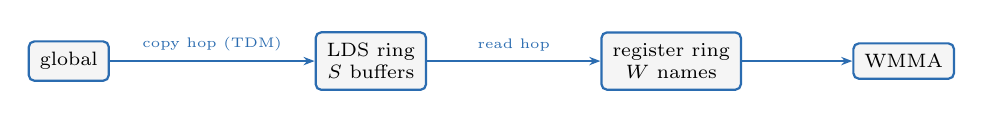
\begin{tikzpicture}
  \node[box] (g) {global};
  \node[box, right=26mm of g] (l) {LDS ring\\$S$ buffers};
  \node[box, right=22mm of l] (r) {register ring\\$W$ names};
  \node[box, right=14mm of r] (c) {WMMA};
  \draw[ar] (g) -- node[above,font=\tiny,text=acc]{copy hop (TDM)} (l);
  \draw[ar] (l) -- node[above,font=\tiny,text=acc]{read hop} (r);
  \draw[ar] (r) -- (c);
\end{tikzpicture}
\end{center}

\begin{columns}[T]
\column{0.50\textwidth}
{\scriptsize \textbf{Per op-class, per hop, the decoder must decide:}}
\begin{itemize}\scriptsize
  \item at \key{which loop level} the operation lives
  \item \key{how far ahead} of its consumer it runs \tsub{(retime $\mathit{off}$, peel depth $M$)}
  \item \key{which rotating buffer} this access touches
  \item where the \key{read pointer flips} and the \key{descriptor advances}
  \item what \key{completion counter} it waits on
  \item where the \key{fence} goes
\end{itemize}

\column{0.46\textwidth}
{\scriptsize \textbf{Times a parameter space that ships:}}
\begin{itemize}\scriptsize
  \item six 3-letter loop orders, plus 6-letter interleaved words \tsub{(96 accepted spellings, 90 distinct traversals; only the 6 doubled words collapse, so 84 are non-contiguous)}
  \item prefetch depths, tile splits per operand \emph{and} per axis, wave count, bf16 / f8 / MX-scaled f8
  \item \key{5{,}744} bf16, \key{152} f8, \key{404--444} mxf8 kernels in the shipping matrices
\end{itemize}
\end{columns}

\vspace{2mm}
{\scriptsize \bad{Six answers, given implicitly, by where a call sits in a Python function.} No layer
owned any of them, so each new parameter interacted with all six at once --- and a wrong answer showed
up as a numeric miscompare on hardware, not as a failure at the point of the decision.}

\end{frame}

% ==== frames/010_02.tex
\begin{frame}{The answer is three layers, and each is defined as much by what it is forbidden to know}

\begin{center}
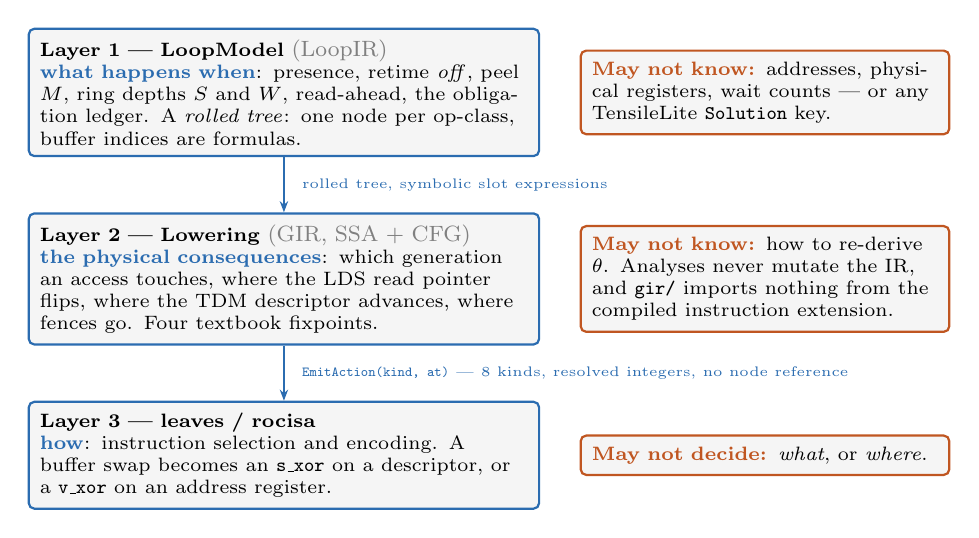
\begin{tikzpicture}[node distance=4mm]
  \node[box, text width=62mm, align=left] (a1)
    {\textbf{Layer 1 --- LoopModel} \tsub{(LoopIR)}\\
     \key{what happens when}: presence, retime $\mathit{off}$, peel $M$, ring depths $S$ and $W$,
     read-ahead, the obligation ledger. A \emph{rolled tree}: one node per op-class, buffer indices
     are formulas.};
  \node[wbox, text width=44mm, align=left, right=5mm of a1] (b1)
    {\bad{May not know:} addresses, physical registers, wait counts --- or any TensileLite
     \texttt{Solution} key.};

  \node[box, text width=62mm, align=left, below=7mm of a1] (a2)
    {\textbf{Layer 2 --- Lowering} \tsub{(GIR, SSA + CFG)}\\
     \key{the physical consequences}: which generation an access touches, where the LDS read
     pointer flips, where the TDM descriptor advances, where fences go. Four textbook fixpoints.};
  \node[wbox, text width=44mm, align=left, right=5mm of a2] (b2)
    {\bad{May not know:} how to re-derive $\theta$. Analyses never mutate the IR, and \texttt{gir/}
     imports nothing from the compiled instruction extension.};

  \node[box, text width=62mm, align=left, below=7mm of a2] (a3)
    {\textbf{Layer 3 --- leaves / rocisa}\\
     \key{how}: instruction selection and encoding. A buffer swap becomes an \texttt{s\_xor} on a
     descriptor, or a \texttt{v\_xor} on an address register.};
  \node[wbox, text width=44mm, align=left, right=5mm of a3] (b3)
    {\bad{May not decide:} \emph{what}, or \emph{where}.};

  \draw[ar] (a1) -- node[right,font=\tiny,text=acc,xshift=1mm]{rolled tree, symbolic slot expressions} (a2);
  \draw[ar] (a2) -- node[right,font=\tiny,text=acc,xshift=1mm]{\texttt{EmitAction(kind, at)} --- 8 kinds, resolved integers, no node reference} (a3);
\end{tikzpicture}
\end{center}

\vspace{1mm}
{\scriptsize \key{The forbidden column is the load-bearing one.} Each boundary is enforced, not
merely intended: the schedule model reads no \texttt{Solution} key, the dataflow IR imports nothing
from the instruction extension, and the leaves receive resolved integers with no node reference to
follow back. A layer that cannot see the next one's inputs cannot silently take over its decision.}

\end{frame}

% ==== frames/010_02b.tex
\begin{frame}{The through-line, and the map: the schedule model decides WHEN, the dataflow IR resolves WHERE}

\begin{center}
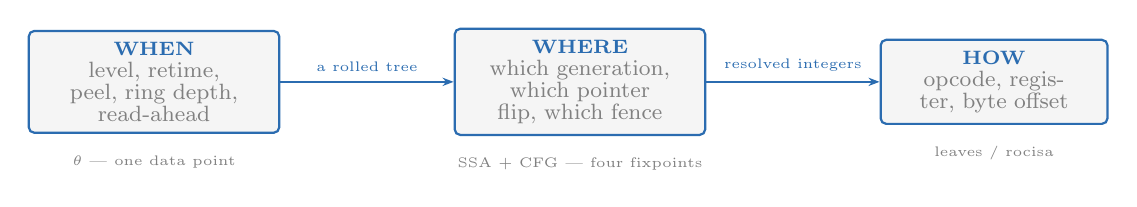
\begin{tikzpicture}[font=\scriptsize,node distance=6mm]
\node[box,text width=2.9cm] (w) {\key{WHEN}\\\tsub{level, retime, peel, ring depth, read-ahead}};
\node[box,text width=2.9cm,right=22mm of w] (e) {\key{WHERE}\\\tsub{which generation, which pointer flip, which fence}};
\node[box,text width=2.6cm,right=22mm of e] (h) {\key{HOW}\\\tsub{opcode, register, byte offset}};
\draw[ar] (w) -- node[above,font=\tiny,text=acc]{a rolled tree} (e);
\draw[ar] (e) -- node[above,font=\tiny,text=acc]{resolved integers} (h);
\node[below=1.5mm of w,font=\tiny,text=gray] {$\theta$ --- one data point};
\node[below=1.5mm of e,font=\tiny,text=gray] {SSA + CFG --- four fixpoints};
\node[below=1.5mm of h,font=\tiny,text=gray] {leaves / rocisa};
\end{tikzpicture}
\end{center}

\vspace{2mm}
{\footnotesize The split is not tidiness. Each layer prevents a failure the other cannot see:
a \key{schedule} question asked of a dataflow pass has no point to reach and no value to
propagate; a \key{placement} question asked of the schedule model is answered by position in a
function, which is where every defect in this deck came from.}

\vspace{3mm}
{\scriptsize
\begin{tabular}{@{}llp{0.52\textwidth}@{}}
\toprule
\textbf{chapters} & \textbf{layer} & \textbf{the question each answers} \\
\midrule
2--4 \tsub{schedule model; placement; hazards} & WHEN & what exists, how far ahead it runs, and what it owes \\
5--7 \tsub{why a second IR; analyses; passes} & WHERE & which buffer, which flip, which fence --- and how each is proved \\
8 \tsub{address geometry} & HOW & the one thing the model is forbidden to know \\
9--10 \tsub{what shipped; what is next} & --- & the measured trajectory, and the named gaps \\
\bottomrule
\end{tabular}}

\end{frame}

% ==== frames/010_02d.tex
% Copyright Advanced Micro Devices, Inc., or its affiliates.
% SPDX-License-Identifier: MIT
\begin{frame}{Nine words this deck needs --- none of them mean what they mean elsewhere}

{\scriptsize Every noun below is defined by this work. The rest of the deck is these nine, one
concept per frame, in the order a schedule is actually built. \tsub{Return here whenever a term
stops carrying its weight.}}

\vspace{1.5mm}
\begin{columns}[T,onlytextwidth]
\begin{column}{0.49\textwidth}
{\scriptsize\setlength{\tabcolsep}{3pt}
\begin{tabular}{@{}p{0.30\linewidth}p{0.66\linewidth}@{}}
\toprule
\multicolumn{2}{@{}l}{\textbf{\color{acc}WHEN --- the schedule model}}\\
\midrule
\key{$\theta$} & one schedule, as seven fields. A \emph{point} in a space, not a program \\[2pt]
\key{op-class} & one operand $\times$ one hop. The unit everything is keyed on \\[2pt]
\key{presence} & the inner axes an op-class varies over. \emph{Derived}, never declared \\[2pt]
\key{retime (off)} & how many steps ahead of its consumer an op-class runs \\[2pt]
\key{ring ($S$, $W$)} & the rotating buffers a hop lands in; \texttt{slot = coordinate mod $S$} \\
\bottomrule
\end{tabular}}
\end{column}
\begin{column}{0.49\textwidth}
{\scriptsize\setlength{\tabcolsep}{3pt}
\begin{tabular}{@{}p{0.30\linewidth}p{0.66\linewidth}@{}}
\toprule
\multicolumn{2}{@{}l}{\textbf{\color{acc}WHEN --- the proof}}\\
\midrule
\key{obligation} & a named hazard: ``X must finish before Y''. Listed \emph{before} any code exists \\[4pt]
\multicolumn{2}{@{}l}{\textbf{\color{acc}WHERE --- the dataflow IR}}\\
\midrule
\key{generation} & which rotation of a ring an access touches --- an \emph{SSA value} \\[2pt]
\key{Mark} & a semantic fact placed at a program point, with a legal \emph{range} \\[2pt]
\key{memory token} & an LDS pseudo-register. Same token = may alias, order them \\
\bottomrule
\end{tabular}}
\end{column}
\end{columns}

\vspace{2mm}
\begin{center}
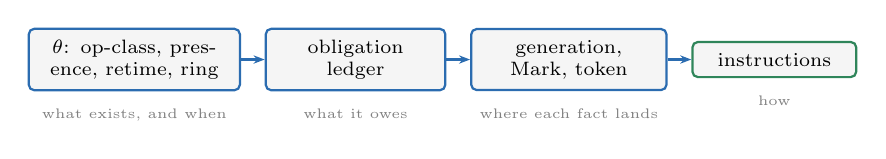
\begin{tikzpicture}[font=\scriptsize,node distance=3mm]
\node[box,text width=2.4cm] (a) {$\theta$: op-class, presence, retime, ring};
\node[box,right=of a,text width=2.0cm] (b) {obligation ledger};
\node[box,right=of b,text width=2.2cm] (c) {generation, Mark, token};
\node[gbox,right=of c,text width=1.8cm] (d) {instructions};
\draw[ar](a)--(b); \draw[ar](b)--(c); \draw[ar](c)--(d);
\node[below=1mm of a,font=\tiny,text=gray]{what exists, and when};
\node[below=1mm of b,font=\tiny,text=gray]{what it owes};
\node[below=1mm of c,font=\tiny,text=gray]{where each fact lands};
\node[below=1mm of d,font=\tiny,text=gray]{how};
\end{tikzpicture}
\end{center}

\end{frame}

% ==== frames/010_02c.tex
\begin{frame}{Where this deck goes --- one concept per frame, then the evidence}
\vspace{-1mm}
\begin{columns}[T,onlytextwidth]
\begin{column}{0.52\textwidth}
\textbf{\color{acc}Decides WHEN} \tsub{— the schedule model}\\[1mm]
{\scriptsize
\begin{tabular}{@{}rp{0.78\linewidth}@{}}
\tsub{2} & \textbf{What a schedule IS} — seven fields, op-class, presence, rings\\
\tsub{3} & \textbf{Placement} — retiming a schedule into a pipeline\\
\tsub{4} & \textbf{Obligations} — the correctness argument\\
\end{tabular}}

\vspace{2.5mm}
\textbf{\color{acc}Resolves WHERE} \tsub{— the dataflow IR}\\[1mm]
{\scriptsize
\begin{tabular}{@{}rp{0.78\linewidth}@{}}
\tsub{5} & \textbf{Why a second IR} — and what a tree cannot answer\\
\tsub{6} & \textbf{The analyses} — generations, tokens, hazards, fences\\
\tsub{7} & \textbf{Passes and verification} — and the emission boundary\\
\end{tabular}}

\vspace{2.5mm}
\textbf{\color{acc}Decides HOW} \tsub{— the leaves}\\[1mm]
{\scriptsize
\begin{tabular}{@{}rp{0.78\linewidth}@{}}
\tsub{8} & \textbf{Address geometry} — the one thing the model may not know\\
\end{tabular}}

\vspace{2.5mm}
\textbf{\color{acc}Evidence}\\[1mm]
{\scriptsize
\begin{tabular}{@{}rp{0.78\linewidth}@{}}
\tsub{9} & \textbf{What shipped}, and how it is validated\\
\tsub{10} & \textbf{Known gaps}, and the bet this design makes\\
\end{tabular}}
\end{column}

\begin{column}{0.46\textwidth}
\vspace{1mm}
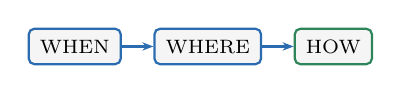
\begin{tikzpicture}
  \node[box](w){WHEN};
  \node[box,right=4mm of w](r){WHERE};
  \node[gbox,right=4mm of r](h){HOW};
  \draw[ar](w)--(r); \draw[ar](r)--(h);
\end{tikzpicture}\\
\tsub{Each layer is forbidden to know the next one's answer.}

\vspace{4mm}
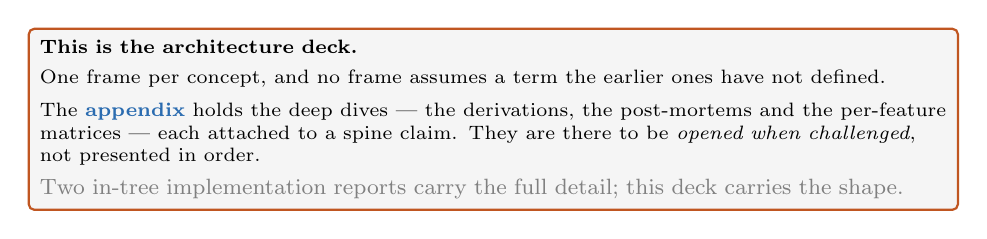
\begin{tikzpicture}
\node[wbox,text width=0.95\columnwidth,align=left]{%
\scriptsize\textbf{This is the architecture deck.}\\[3pt]
\raggedright
One frame per concept, and no frame assumes a term the earlier ones have not defined.\\[4pt]
The \key{appendix} holds the deep dives — the derivations, the post-mortems and the
per-feature matrices — each attached to a spine claim. They are there to be \emph{opened when
challenged}, not presented in order.\\[4pt]
\tsub{Two in-tree implementation reports carry the full detail; this deck carries the shape.}};
\end{tikzpicture}
\end{column}
\end{columns}
\end{frame}

\section{The schedule model -- what a schedule IS}
% ==== frames/020_01.tex

\begin{frame}{A schedule is seven fields --- and deliberately none of them is an address}
\begin{columns}[T]
\begin{column}{0.5\textwidth}
\vspace{2pt}
\begin{center}
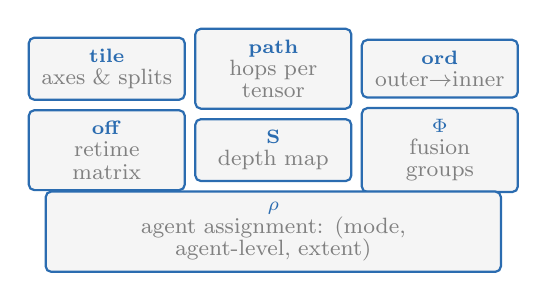
\begin{tikzpicture}[font=\tiny,node distance=3pt]
\node[box,text width=1.7cm] (t) {\key{tile}\\\tsub{axes \& splits}};
\node[box,right=of t,text width=1.7cm] (p) {\key{path}\\\tsub{hops per tensor}};
\node[box,right=of p,text width=1.7cm] (o) {\key{ord}\\\tsub{outer$\to$inner}};
\node[box,below=of t,text width=1.7cm] (f) {\key{off}\\\tsub{retime matrix}};
\node[box,below=of p,text width=1.7cm] (s) {\key{S}\\\tsub{depth map}};
\node[box,below=of o,text width=1.7cm] (ph) {\key{$\Phi$}\\\tsub{fusion groups}};
\node[box,below=of s,text width=5.5cm] (r)
  {\key{$\rho$}\\\tsub{agent assignment: (mode, agent-level, extent)}};
\end{tikzpicture}
\end{center}
\end{column}
\begin{column}{0.48\textwidth}
\vspace{-2pt}
\begin{itemize}\itemsep2pt
\item \key{S} is \emph{derived}, not authored.
\item \key{off} is keyed by \emph{op-class} $\times$ \emph{level} --- not by operand.
\item \key{$\Phi$} merges op-classes into one cooperative instruction; members pair \emph{by region index},
      and the two operands may be cut on different axes.
\item \key{$\rho$ is a \emph{map}} --- which mode each \emph{agent level} traverses instead of the
      coordinate, over how many agents --- and the \key{single} agent authority. $\Phi$ over
      $\rho$ is what turns a wide load into a \key{broadcast}.
\end{itemize}
\vspace{4pt}
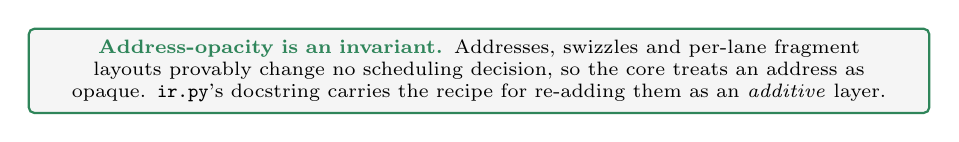
\begin{tikzpicture}
\node[gbox,text width=0.92\textwidth]{\good{Address-opacity is an invariant.}
Addresses, swizzles and per-lane fragment layouts provably change no scheduling decision,
so the core treats an address as opaque. \texttt{ir.py}'s docstring carries the recipe for
re-adding them as an \emph{additive} layer.};
\end{tikzpicture}
\end{column}
\end{columns}
\end{frame}

% ==== frames/020_02.tex
\begin{frame}{Everything is keyed on the op-class --- so presence is a per-hop fact, not a per-operand one}
\begin{center}
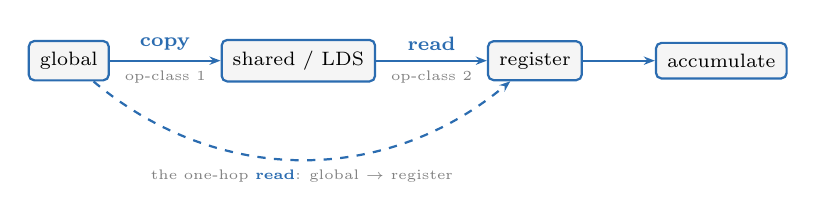
\begin{tikzpicture}[font=\scriptsize,node distance=10pt]
\node[box] (g) {global};
\node[box,right=40pt of g] (l) {shared / LDS};
\node[box,right=40pt of l] (v) {register};
\node[box,right=26pt of v] (c) {accumulate};
\draw[ar] (g) -- node[above,font=\scriptsize]{\key{copy}} node[below,font=\tiny,text=gray]{op-class 1} (l);
\draw[ar] (l) -- node[above,font=\scriptsize]{\key{read}} node[below,font=\tiny,text=gray]{op-class 2} (v);
\draw[ar] (v) -- (c);
\draw[ar,dashed] (g) to[out=-40,in=-140]
  node[below,font=\tiny,text=gray,pos=0.5]{the one-hop \key{read}: global $\to$ register} (v);
\end{tikzpicture}
\end{center}
\vspace{2pt}
\begin{columns}[T]
\begin{column}{0.46\textwidth}
\textbf{An op-class = one operand, one hop.}
\begin{itemize}\itemsep1pt
\item \key{role} $\in$ \{copy, read, store\}, from one table.
\item \key{trajectory} is separate: in a store round trip the middle leg's \emph{role} is
      \texttt{read} while its \emph{sense} is reverse.
\item \texttt{off}, the ledger's endpoints and the emitted tree all name op-classes.
\end{itemize}
\end{column}
\begin{column}{0.52\textwidth}
\textbf{Presence} = the inner axes an op-class varies over.
\begin{center}\scriptsize
\begin{tabular}{@{}lc@{}}
\toprule
hop & presence \\
\midrule
bulk cooperative copy & $\emptyset$ \tsub{(sits at the chunk)} \\
same copy, tile cut into $n$ regions & \{region axis\} \\
per-lane read & the operand's data axes \\
\bottomrule
\end{tabular}
\end{center}
\vspace{2pt}
\bad{Same operand, different answers.} Asking the operand instead of the hop puts a bulk copy
at the wrong level --- and a region split is what brings the axis back.
\end{column}
\end{columns}
\end{frame}

% ==== frames/020_03.tex
\begin{frame}[fragile]{Reduction axes are derived by subtraction --- which is exactly why a third class was needed}
\begin{center}
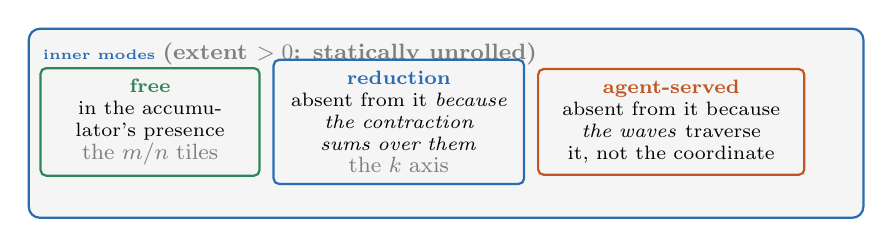
\begin{tikzpicture}[font=\scriptsize]
\node[draw=acc,thick,rounded corners,minimum width=10.6cm,minimum height=2.4cm,fill=lt] (all) {};
\node[anchor=north west,font=\tiny\bfseries,text=acc] at ([shift={(2pt,-2pt)}]all.north west)
  {inner modes \tsub{(extent $>0$: statically unrolled)}};
\node[gbox,below right=0.5cm and 0.15cm of all.north west,text width=2.5cm] (free)
  {\good{free}\\ in the accumulator's presence\\ \tsub{the $m$/$n$ tiles}};
\node[box,right=0.15cm of free,text width=2.9cm] (red)
  {\key{reduction}\\ absent from it \emph{because the contraction sums over them}\\ \tsub{the $k$ axis}};
\node[wbox,right=0.15cm of red,text width=3.1cm] (ag)
  {\bad{agent-served}\\ absent from it because \emph{the waves} traverse it, not the coordinate};
\end{tikzpicture}
\end{center}
\vspace{-2pt}
\begin{columns}[T]
\begin{column}{0.5\textwidth}
\textbf{Defined at one point, not at each consumer:}
\begin{lstlisting}[style=pseudo]
reduction = inner
          \ presence(each output op-class)
          \ agent_served
free(op)  = presence(op) \ reduction
\end{lstlisting}
\end{column}
\begin{column}{0.47\textwidth}
\textbf{An axis is agent-served when, for some operand:}
\begin{itemize}\itemsep0pt
\item it has region modes, \emph{and}
\item the region split is $>1$ --- having an axis is not having two of them, \emph{and}
\item some \key{non-bulk} hop is agent-relative.
\end{itemize}
\vspace{2pt}
The bulk copy still walks every region by index; only the \emph{read} is agent-relative.
That asymmetry is the whole class.
\end{column}
\end{columns}
\end{frame}

% ==== frames/020_05.tex
\begin{frame}{Extent alone tells outer from inner --- one field, so a new loop level is not a new decoder branch}
\begin{center}
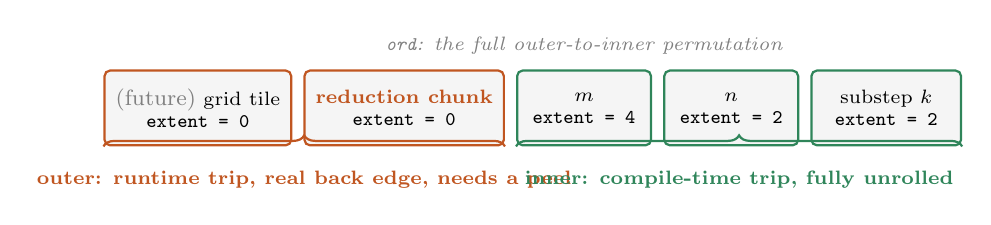
\begin{tikzpicture}[font=\scriptsize]
\node[wbox,minimum width=2.2cm,minimum height=0.95cm] (o1) {\tsub{(future)} grid tile\\\texttt{extent = 0}};
\node[box,right=4pt of o1,minimum width=2.4cm,minimum height=0.95cm,draw=warn] (o2) {\bad{reduction chunk}\\\texttt{extent = 0}};
\node[gbox,right=4pt of o2,minimum width=1.7cm,minimum height=0.95cm] (i1) {$m$\\\texttt{extent = 4}};
\node[gbox,right=4pt of i1,minimum width=1.7cm,minimum height=0.95cm] (i2) {$n$\\\texttt{extent = 2}};
\node[gbox,right=4pt of i2,minimum width=1.9cm,minimum height=0.95cm] (i3) {substep $k$\\\texttt{extent = 2}};
\draw[decorate,decoration={brace,amplitude=4pt},draw=warn,thick]
  (o1.south west) -- (o2.south east) node[midway,below=5pt,text=warn,font=\scriptsize\bfseries]{outer: runtime trip, real back edge, needs a peel};
\draw[decorate,decoration={brace,amplitude=4pt},draw=ok,thick]
  (i1.south west) -- (i3.south east) node[midway,below=5pt,text=ok,font=\scriptsize\bfseries]{inner: compile-time trip, fully unrolled};
\node[above=2pt of i1,font=\scriptsize\itshape,text=gray] {\texttt{ord}: the full outer-to-inner permutation};
\end{tikzpicture}
\end{center}
\vspace{6pt}
\begin{columns}[T]
\begin{column}{0.5\textwidth}
\begin{itemize}\itemsep2pt
\item Shared ring rotates \emph{across} the outer levels; register ring rotates \emph{inside} the inner ones.
\item \texttt{ord} is a permutation $\Rightarrow$ any subset traverses as a \key{monotone mixed-radix counter};
      a mode's stride is the product of the extents inner to it.
\end{itemize}
\end{column}
\begin{column}{0.48\textwidth}
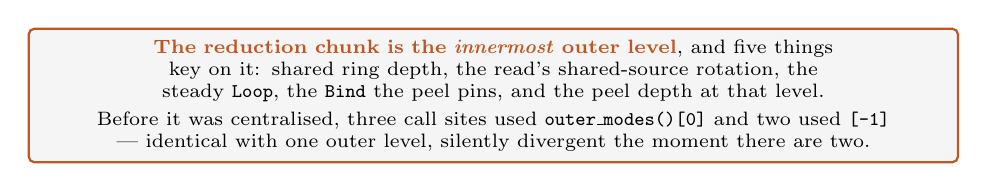
\begin{tikzpicture}
\node[wbox,text width=0.95\textwidth]{\bad{The reduction chunk is the \emph{innermost} outer level}, and five things
key on it: shared ring depth, the read's shared-source rotation, the steady \texttt{Loop},
the \texttt{Bind} the peel pins, and the peel depth at that level.\\[2pt]
Before it was centralised, three call sites used \texttt{outer\_modes()[0]} and two used \texttt{[-1]}
--- identical with one outer level, silently divergent the moment there are two.};
\end{tikzpicture}
\end{column}
\end{columns}
\end{frame}

% ==== frames/020_07.tex
\begin{frame}{Two rings, one rule: \texttt{slot = coordinate mod S} --- what differs is which coordinate turns}
\begin{columns}[T]
\begin{column}{0.44\textwidth}
\begin{center}
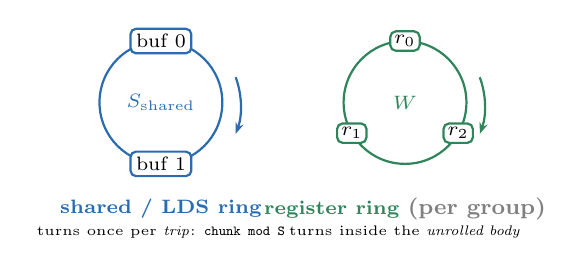
\begin{tikzpicture}[font=\tiny]
% shared ring
\draw[thick,draw=acc] (0,0) circle (0.78);
\node[box,fill=white,inner sep=2pt] at (0,0.78) {buf 0};
\node[box,fill=white,inner sep=2pt] at (0,-0.78) {buf 1};
\draw[ar,draw=acc] (0.95,0.32) arc (20:-20:1.05);
\node[font=\scriptsize,text=acc] at (0,0) {$S_{\text{shared}}$};
\node[font=\scriptsize\bfseries,text=acc] at (0,-1.35) {shared / LDS ring};
\node at (0,-1.65) {turns once per \emph{trip}: \texttt{chunk mod S}};
% register ring
\begin{scope}[xshift=3.1cm]
\draw[thick,draw=ok] (0,0) circle (0.78);
\node[gbox,fill=white,inner sep=1.5pt] at (90:0.78) {$r_0$};
\node[gbox,fill=white,inner sep=1.5pt] at (210:0.78) {$r_1$};
\node[gbox,fill=white,inner sep=1.5pt] at (330:0.78) {$r_2$};
\draw[ar,draw=ok] (0.95,0.32) arc (20:-20:1.05);
\node[font=\scriptsize,text=ok] at (0,0) {$W$};
\node[font=\scriptsize\bfseries,text=ok] at (0,-1.35) {register ring \tsub{(per group)}};
\node at (0,-1.65) {turns inside the \emph{unrolled body}};
\end{scope}
\end{tikzpicture}
\end{center}
\end{column}
\begin{column}{0.55\textwidth}
\vspace{-4pt}
\begin{center}\scriptsize
\begin{tabular}{@{}p{1.5cm}p{2.0cm}p{2.2cm}@{}}
\toprule
& shared ring & register ring \\
\midrule
coordinate & reduction chunk index & mixed-radix index over the group's \emph{rate modes} \\
modulus & $S_{\text{shared}}$: a \key{target fact} (the LDS allocation) & $W$: \key{searched} in a derived band $[L, R]$ \\
generation & one chunk of an operand in one buffer & one filling of one register name \\
\bottomrule
\end{tabular}
\end{center}
\vspace{1pt}
\begin{itemize}\itemsep1pt
\item $W<L$ is a race, $W>R$ is waste. $W=1$ is in-place: safety comes from \emph{ordering}, not capacity.
\item Both slots stay symbolic \texttt{Expr}s, so the tree stays rolled.
\end{itemize}
\vspace{2pt}
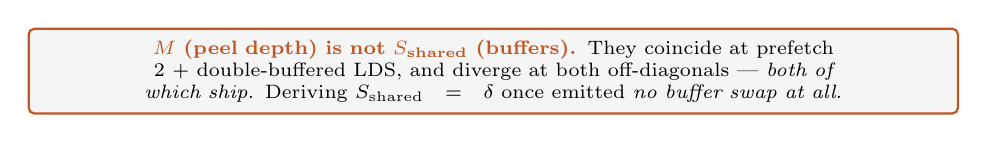
\begin{tikzpicture}
\node[wbox,text width=0.95\textwidth]{\bad{$M$ (peel depth) is not $S_{\text{shared}}$ (buffers).}
They coincide at prefetch 2 + double-buffered LDS, and diverge at both off-diagonals
--- \emph{both of which ship}. Deriving $S_{\text{shared}}=\delta$ once emitted \emph{no buffer swap at all}.};
\end{tikzpicture}
\end{column}
\end{columns}
\end{frame}

\section{Placement -- turning a schedule into a pipeline}
% ==== frames/030_01.tex

\begin{frame}{Retiming is one integer per op-class; it costs two peels and a fallback arm}

\begin{center}
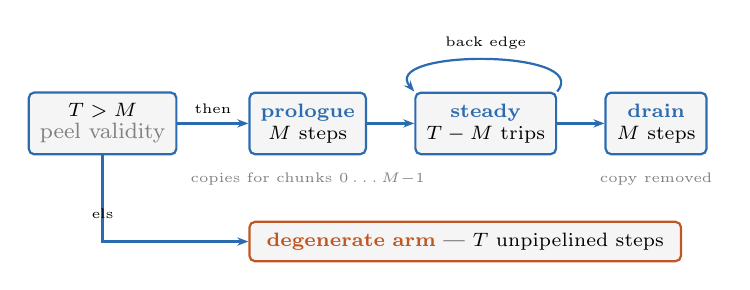
\begin{tikzpicture}[font=\scriptsize,node distance=6mm]
  \node[box] (g) {$T > M$\\\tsub{peel validity}};
  \node[box,right=9mm of g] (pro) {\key{prologue}\\$M$ steps};
  \node[box,right=6mm of pro] (st) {\key{steady}\\$T-M$ trips};
  \node[box,right=6mm of st] (dr) {\key{drain}\\$M$ steps};
  \node[wbox,below=15mm of pro.west,anchor=west,text width=52mm] (sh)
       {\bad{degenerate arm} --- $T$ unpipelined steps};
  \draw[ar] (g) -- node[above,font=\tiny]{then} (pro);
  \draw[ar] (pro) -- (st);
  \draw[ar] (st) -- (dr);
  \draw[ar] (st.north east) to[out=50,in=130] node[above,font=\tiny]{back edge} (st.north west);
  \draw[ar] (g.south) |- node[below,font=\tiny,pos=0.25]{els} (sh.west);
  \node[font=\tiny,gray,below=1mm of pro] {copies for chunks $0\dots M{-}1$};
  \node[font=\tiny,gray,below=1mm of dr] {copy removed};
\end{tikzpicture}
\end{center}

\begin{itemize}
  \item $\mathrm{off}(c,\text{chunk})=\delta$ means \emph{chunk $i$'s copy is issued in iteration $i-\delta$}. That is the whole of software pipelining, as one integer. $M=\max_p \delta_p$.
  \item The peel is \key{staggered, not uniform}: $\mathrm{copy}_p$ is present at prologue step $t$ iff $\delta_p \ge M-t$, and at drain step $t$ iff $\delta_p \le M-1-t$ --- deepest in first, deepest out first.
  \item The guard is \key{strictly} $T>M$. The steady region lowers to a \emph{post-tested} block, which cannot express zero trips; under $\ge$, $T=M$ would run one trip computing chunk 0 that the drain also computes.
  \item Consequence taken deliberately: the short arm is \bad{live code at every peel depth}, not dead at depth 1.
\end{itemize}
\end{frame}

% ==== frames/030_02.tex
\begin{frame}[fragile]{A read hoisted $d$ steps buys latency hiding and owes three things back}

Issued naively, every read is followed by a wait for its own completion: the machine stalls the full
local-memory latency at each step. Hoisting the read $d$ steps creates three obligations --- and each
is a \key{closed form}, never a simulation.

\begin{center}
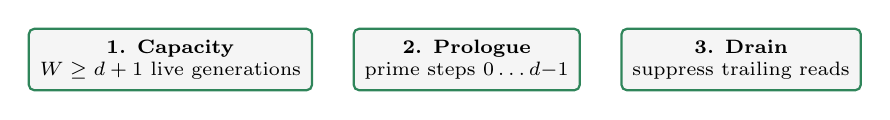
\begin{tikzpicture}[font=\scriptsize]
  \node[gbox] (cap) {\textbf{1. Capacity}\\$W \ge d+1$ live generations};
  \node[gbox,right=5mm of cap] (pro) {\textbf{2. Prologue}\\prime steps $0\dots d{-}1$};
  \node[gbox,right=5mm of pro] (drn) {\textbf{3. Drain}\\suppress trailing reads};
\end{tikzpicture}
\end{center}

\begin{lstlisting}[style=pseudo]
dr   = off(read, substep)                 # the REQUEST, per op-class
dr_g = 0  if fan(op) > 1                                        [veto 1]
       0  if a free sibling is outer to the group's reduction   [veto 2]
       max(0, min(dr, W_g - 1))                    # the capacity clamp
\end{lstlisting}

\begin{center}\scriptsize
\begin{tabular}{lll}
\toprule
 & \good{Shape A} ($dr_g \ge 1$) & \bad{Shape B} ($dr_g = 0$) \\
\midrule
read placement & hoisted ahead of its consumer & in place, with a wait \\
prologue       & non-empty & \textbf{empty} \\
steady advance & non-zero  & \textbf{0} \\
\bottomrule
\end{tabular}
\end{center}

\tsub{Mixing them is what the \texttt{dr\_g} refactor exists to prevent --- and was the decoder's real state: a Shape-A prologue with a Shape-B steady primes the pipe once and never re-primes it.}
\end{frame}

% ==== frames/030_04.tex
\begin{frame}{The peel is a vector over levels --- and one offset relocates instead of peeling}

The retime matrix is indexed by \key{(op-class, level)}, so \emph{any} level can carry an offset: an
outer tile level, the reduction chunk, the substep. \texttt{PeelDepths} therefore reports
$M_\ell$ per level, the per-op-class offsets, the substep request, the derived reach, and every
negative offset separately as a deferral.

\begin{itemize}
  \item \texttt{PeelDepths.M} is deliberately \key{narrow} --- the chunk level, the only one whose prologue/drain the emitter can build --- and sits beside \texttt{peeled\_levels()}, which reports \emph{all} of them. That pairing turns a silent drop into a loud refusal.
  \item It used to return an \texttt{int} keyed on the chunk. The tree stayed well formed, the ledger came back empty, and the certificate \bad{certified a schedule nobody requested}.
\end{itemize}

\textbf{The cross-level boundary term.} An offset at outer level $\ell$ whose op-class lives strictly
\emph{inside} $\ell$ does not peel $\ell$ --- it relocates the leading $\delta$ instances into the
previous $\ell$-trip's drain. Three conditions decide it, and the third separates these two:

\begin{center}\scriptsize
\begin{tabular}{lll}
\toprule
offset & home level & verdict \\
\midrule
\texttt{off(copy, gtile)} & \texttt{iter} --- an outer, looped level & \good{relocation}: whole iterations move \\
\texttt{off(copy, iter)}  & \texttt{M\_split} --- an inner unrolled axis & \bad{ordinary prefetch}: the fan stays put \\
\bottomrule
\end{tabular}
\end{center}

\tsub{Without condition 3 the two are conflated --- the first implementation reported a boundary term for every shipping region-split kernel, and the emitter refuses on a non-empty hoist list, so it refused them all.}
\end{frame}

% ==== frames/030_06.tex
\begin{frame}{A Mark has a legal range, not a point --- so the policy travels with the region}

Two registers are \emph{mutated}, not re-derived: the shared read pointer (a ring swap) and the
bulk-copy descriptor. Lowering is split three ways --- \key{analysis} emits pending marks over opaque
anchors, \key{placement} picks a point in the window, \key{apply} is the only IR mutator.

\begin{columns}[T]
\begin{column}{0.56\textwidth}
\begin{center}
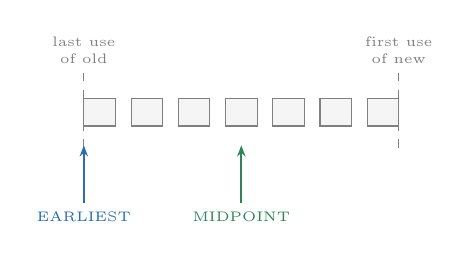
\begin{tikzpicture}[font=\tiny]
  \foreach \i in {0,...,6}{\node[draw=gray,fill=lt,minimum width=4mm,minimum height=3.5mm]
      at (\i*6mm,0) {};}
  \draw[dashed,gray] (-0.2,-0.45) -- (-0.2,0.5);
  \draw[dashed,gray] (3.8,-0.45) -- (3.8,0.5);
  \node[font=\tiny,text=gray,align=center,anchor=south] at (-0.2,0.5) {last use\\of old};
  \node[font=\tiny,text=gray,align=center,anchor=south] at (3.8,0.5) {first use\\of new};
  \draw[ar,draw=acc] (-0.2,-1.15) -- (-0.2,-0.42);
  \node[font=\tiny,text=acc,anchor=north] at (-0.2,-1.15) {EARLIEST};
  \draw[ar,draw=ok] (1.8,-1.15) -- (1.8,-0.42);
  \node[font=\tiny,text=ok,anchor=north] at (1.8,-1.15) {MIDPOINT};
\end{tikzpicture}
\end{center}
\end{column}
\begin{column}{0.42\textwidth}
\begin{center}
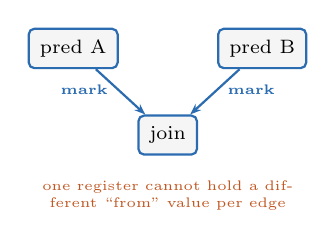
\begin{tikzpicture}[font=\tiny,node distance=5mm]
  \node[box] (p1) at (0,0) {pred A};
  \node[box] (p2) at (2.4,0) {pred B};
  \node[box] (j)  at (1.2,-1.1) {join};
  \draw[ar] (p1) -- node[left,font=\tiny,pos=0.45]{\key{mark}} (j);
  \draw[ar] (p2) -- node[right,font=\tiny,pos=0.45]{\key{mark}} (j);
  \node[font=\tiny,warn,below=2mm of j,text width=32mm,align=center] {one register cannot hold a different ``from'' value per edge};
\end{tikzpicture}
\end{center}
\end{column}
\end{columns}

\begin{itemize}\footnotesize
  \item \key{Descriptor changes go earliest} --- gr\_inc \emph{and} the copy-hop swap, one rule: they mutate one resource and feed one consumer. Every cycle before the load is overlap, and the window's lower bound already \emph{is} the last use of the old value.
  \item \key{The read swap goes at the midpoint} --- bounded by two \emph{different} resources, so either edge stalls against that edge's consumer. Honestly a heuristic: a bisection of the node list, not of a cost model.
  \item \key{One Mark per incoming path} --- an exit def in each predecessor, never one at the join. From an AVAIL/ANTIC fixpoint; \bad{TOP is reported, never resolved}.
\end{itemize}
\end{frame}

\section{Obligations -- the correctness argument}
% ==== frames/040_01.tex

\begin{frame}{The correctness argument is a list written \emph{before} any code exists}

\begin{columns}[T]
\begin{column}{0.46\textwidth}
\vspace{2pt}
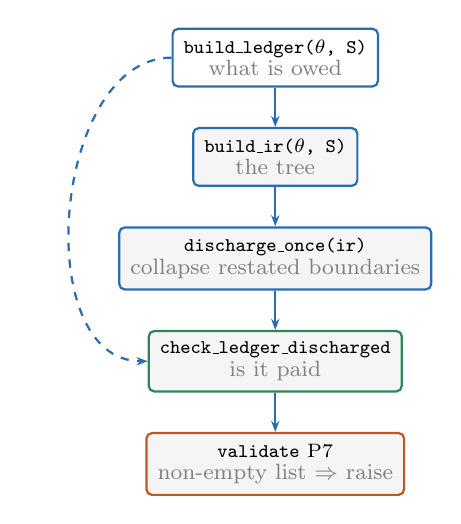
\begin{tikzpicture}[node distance=5mm]
\node[box,fill=white] (l) {\texttt{build\_ledger($\theta$, S)}\\\tsub{what is owed}};
\node[box,below=of l] (e) {\texttt{build\_ir($\theta$, S)}\\\tsub{the tree}};
\node[box,below=of e] (d) {\texttt{discharge\_once(ir)}\\\tsub{collapse restated boundaries}};
\node[gbox,below=of d] (c) {\texttt{check\_ledger\_discharged}\\\tsub{is it paid}};
\node[wbox,below=5mm of c] (p) {\texttt{validate} P7\\\tsub{non-empty list $\Rightarrow$ raise}};
\draw[ar] (l)--(e); \draw[ar] (e)--(d); \draw[ar] (d)--(c); \draw[ar] (c)--(p);
\draw[ar,dashed] (l.west) to[out=180,in=180] (c.west);
\end{tikzpicture}
\end{column}
\begin{column}{0.52\textwidth}
\vspace{2pt}
\key{An obligation is a hazard, named, so it can be tracked to a discharge.}

\vspace{2pt}
{\ttfamily\small Obligation(producer, consumer, kind, counter)}

\vspace{2pt}
\begin{itemize}\itemsep2pt
  \item ends are structured \texttt{Endpoint} records --- op-class, storage/site, role
  \item \texttt{counter} is a \key{completion class} (\texttt{C\_copy}, \texttt{C\_read}), a model label, not a hardware counter
  \item \key{symbolic per op-class}, not per iteration: one row for ``A's global$\to$shared feeds A's shared$\to$register''
\end{itemize}
\vspace{3pt}
The ledger is small enough to be built and checked on \emph{every} decode.
\end{column}
\end{columns}
\end{frame}

% ==== frames/040_03.tex
\begin{frame}{A wait cannot repair an anti-dependency --- the read you need has not issued yet}

\begin{columns}[T]
\begin{column}{0.44\textwidth}
\vspace{2pt}
A completion wait makes an instruction wait for \key{already-issued} operations to finish.

\vspace{4pt}
Ring depth $S_{\text{shared}}$, copy running $\delta$ chunks ahead. At $S_{\text{shared}}=\delta$ the copy of chunk $c+\delta$ lands in slot $c \bmod S_{\text{shared}}$ --- \bad{the slot this trip is reading}.

\vspace{4pt}
Ask what the copy could wait \emph{on} in a \texttt{copy; reads} body: the reads that must precede it \emph{have not issued}. There is nothing to name. The only repair is to \key{move the copy}.

\vspace{6pt}
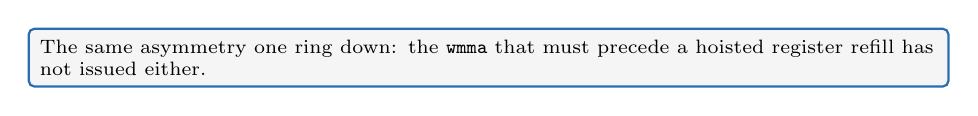
\begin{tikzpicture}
\node[box,text width=0.94\columnwidth,align=left,font=\scriptsize] {The same asymmetry one ring down: the \texttt{wmma} that must precede a hoisted register refill has not issued either.};
\end{tikzpicture}
\end{column}
\begin{column}{0.54\textwidth}
\vspace{-4pt}
\small
\begin{tabular}{@{}p{2.1cm}p{2.0cm}p{3.0cm}@{}}
\toprule
\textbf{Mechanism} & \textbf{Discharges} & \textbf{Enforced by} \\
\midrule
a \key{wait} \tsub{(an \texttt{Await} naming the producer)} & \texttt{RAW-residency}, \texttt{crossing-RAW} & arm (a) coverage; order otherwise free \\[4pt]
a \key{position} \tsub{(the issue order $\sigma_c$)} & \texttt{rotation-WAR}, \texttt{inplace-WAR} & arms (b), (b2), (b3); no wait exists \\[4pt]
mere \key{presence} \tsub{(a read the prologue must contain)} & \texttt{readahead-residency} & arm (c), against the prologue body \\
\bottomrule
\end{tabular}

\vspace{6pt}
\textbf{Presence is not a wait and not an order.} Arm (c) collects the \emph{coordinates} of every register read the prologue emits and requires each obligation's coordinate to be there. A peel built on the wrong reduction axis is rejected \good{at build time} rather than by a passing-or-failing hardware run.

\vspace{4pt}
\tsub{That is also why the fifth kind sits outside the closed set --- it never becomes an \texttt{Await}, so \texttt{is\_war} must never see it.}
\end{column}
\end{columns}
\end{frame}

% ==== frames/040_04.tex
\begin{frame}{``The ledger is empty'' means coverage \emph{and} position --- and nothing about addresses}

\begin{columns}[T]
\begin{column}{0.47\textwidth}
\vspace{2pt}
\good{Two statements per obligation:}
\begin{enumerate}\itemsep3pt
  \item \key{Coverage} --- somewhere in the tree an \texttt{Await} names the obligation's completion class. Otherwise it is unsatisfiable however the code is ordered.
  \item \key{Position} --- within one straight-line trip, the emitted order of producer and consumer is the one the hazard demands.
\end{enumerate}

\vspace{5pt}
Position is not optional \emph{because the backend is order-driven}: it discards the markers and re-derives synchronization from def-use order of the memory tokens. Coverage alone passes an instruction encoding \bad{the inverse dependency}.
\end{column}
\begin{column}{0.50\textwidth}
\vspace{-2pt}
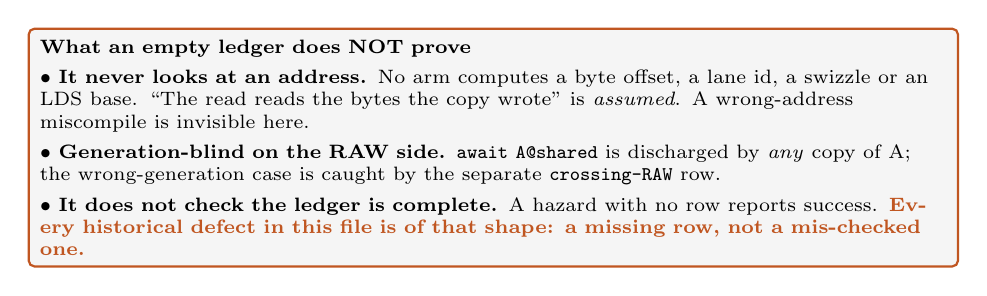
\begin{tikzpicture}
\node[wbox,text width=0.95\columnwidth,align=left] {
\textbf{What an empty ledger does NOT prove}\\[3pt]
\raggedright
$\bullet$~\textbf{It never looks at an address.} No arm computes a byte offset, a lane id, a swizzle or an LDS base. ``The read reads the bytes the copy wrote'' is \emph{assumed}. A wrong-address miscompile is invisible here.\\[3pt]
$\bullet$~\textbf{Generation-blind on the RAW side.} \texttt{await A@shared} is discharged by \emph{any} copy of A; the wrong-generation case is caught by the separate \texttt{crossing-RAW} row.\\[3pt]
$\bullet$~\textbf{It does not check the ledger is complete.} A hazard with no row reports success. \bad{Every historical defect in this file is of that shape: a missing row, not a mis-checked one.}
};
\end{tikzpicture}

\vspace{3pt}
\tsub{The cross-check for the missing-row mode re-derives the shared-memory edge set from the lowered CFG and asserts the two sets are equal.}
\end{column}
\end{columns}
\end{frame}

\section{Why a second IR}
% ==== frames/050_01.tex

\begin{frame}{Four physical questions --- and all four are the same question}
\begin{columns}[T]
\begin{column}{0.56\textwidth}
\begin{enumerate}\scriptsize
  \item Which of the $S$ rotating LDS buffers does \emph{this} access touch?
  \item At which instruction does the LDS \key{read pointer} flip to the next buffer?
  \item At which instruction does the \key{global read address} advance to the next reduction chunk?
  \item Where do \key{barriers} go?
\end{enumerate}
\vspace{4pt}
\scriptsize
Each one reads: \emph{one physical register or resource must hold the right value
at this program point.}
\vspace{3pt}

That is a \good{compiler dataflow problem}, not a scheduling problem --- and the
scheduler is the wrong layer to ask.
\end{column}
\begin{column}{0.42\textwidth}
\centering
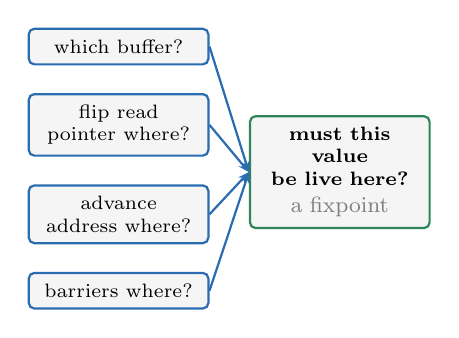
\begin{tikzpicture}[node distance=3.5mm]
  \node[box,text width=2.0cm] (q1) {which buffer?};
  \node[box,text width=2.0cm,below=of q1] (q2) {flip read pointer where?};
  \node[box,text width=2.0cm,below=of q2] (q3) {advance address where?};
  \node[box,text width=2.0cm,below=of q3] (q4) {barriers where?};
  \node[gbox,text width=2.0cm,right=5mm of q2.east,yshift=-6mm]
       (d) {\textbf{must this value\\be live here?}\\[2pt]\tsub{a fixpoint}};
  \foreach \q in {q1,q2,q3,q4} \draw[ar] (\q.east) -- (d.west);
\end{tikzpicture}
\end{column}
\end{columns}
\end{frame}

% ==== frames/050_02.tex
\begin{frame}{A rolled tree has no point to reach and no value to propagate}
\centering
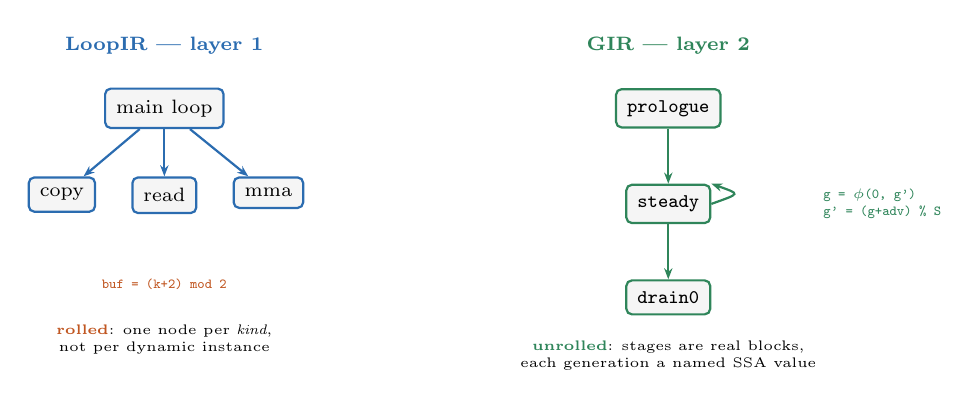
\begin{tikzpicture}[node distance=4mm,every node/.style={font=\scriptsize}]
  % ---- left: LoopIR tree
  \node[box] (r) {main loop};
  \node[box,below left=6mm and 1mm of r] (c) {copy};
  \node[box,below=6mm of r] (l) {read};
  \node[box,below right=6mm and 1mm of r] (m) {mma};
  \foreach \x in {c,l,m} \draw[ar] (r) -- (\x);
  \node[below=7mm of l,align=center,font=\tiny\ttfamily,text=warn]
       (f) {buf = (k+2) mod 2};
  \node[above=3mm of r,font=\scriptsize\bfseries,text=acc] {LoopIR --- layer 1};
  \node[below=2mm of f,align=center,font=\tiny]
       {\bad{rolled}: one node per \emph{kind},\\not per dynamic instance};

  % ---- right: GIR CFG
  \begin{scope}[xshift=6.4cm]
    \node[gbox] (p) {\texttt{prologue}};
    \node[gbox,below=7mm of p] (s) {\texttt{steady}};
    \node[gbox,below=7mm of s] (d) {\texttt{drain0}};
    \draw[ar,draw=ok] (p) -- (s);
    \draw[ar,draw=ok] (s) -- (d);
    \draw[ar,draw=ok] (s.east) to[out=20,in=-20,looseness=4] (s.north east);
    \node[right=13mm of s,align=left,font=\tiny\ttfamily,text=ok]
      {g = $\phi$(0, g')\\g' = (g+adv) \% S};
    \node[above=3mm of p,font=\scriptsize\bfseries,text=ok] {GIR --- layer 2};
    \node[below=2mm of d,align=center,font=\tiny]
      {\good{unrolled}: stages are real blocks,\\each generation a named SSA value};
  \end{scope}
\end{tikzpicture}

\vspace{4pt}
\scriptsize
Unroll the pipeline stages into basic blocks, give every buffer generation a
$\phi$ at the loop header --- and all four questions become \key{textbook fixpoints}.
\emph{That} is the reason for two IRs, not layering for its own sake.
\end{frame}

% ==== frames/050_03.tex
\begin{frame}{The node set is semantic: a swap is a fact, never an \texttt{s\_xor}}
\centering\scriptsize
\begin{tabular}{@{}llp{5.2cm}@{}}
\toprule
group & nodes & answers \\
\midrule
nouns   & \texttt{Tile}, \texttt{Gen}, \texttt{Ref} & what data / which buffer generation / one use of it \\
verbs   & \texttt{Move}, \texttt{Mma} & one movement hop / one multiply--accumulate \\
point   & \texttt{Mark} & a semantic fact at a program point \\
control & \texttt{Goto}, \texttt{CondGoto}, \texttt{LoopBack}, \texttt{Return}, \texttt{CondChain} & the CFG terminators \\
graph   & \texttt{Block}, \texttt{GenPhi}, \texttt{GenXfer}, \texttt{Program} & the CFG itself \\
\bottomrule
\end{tabular}

\vspace{5pt}
\begin{itemize}\scriptsize
  \item \key{No physical fields} (checked by \texttt{G-SEMANTIC}): no address, no VGPR colour,
        no byte offset. The same fact realizes as a descriptor \texttt{s\_xor}, an address
        \texttt{v\_xor}, or nothing at all --- a node naming one cannot be reused by the others.
  \item \key{One SSA value class}: \texttt{Gen}, the loop-carried buffer generation. Registers are
        \emph{not} SSA --- their rotation width is a schedule decision this layer only validates.
  \item \key{Six \texttt{Mark} kinds}, closed set --- and \bad{no \texttt{barrier} kind}: GIR carries the
        ordering obligation, layer 3 picks \texttt{s\_barrier} / a wait count / nothing.
        \tsub{(The comment explaining this is one rename stale --- it still says \texttt{await}.)}
\end{itemize}
\end{frame}

\section{The analyses -- what dataflow buys}
% ==== frames/060_02.tex
\begin{frame}{The pointer is one register and the program is one execution --- so it is ONE timeline, not three regions}
\begin{columns}[T]
\begin{column}{0.44\textwidth}
\footnotesize
\bad{Three seam defects, all shipped, all silent:}
\begin{enumerate}\itemsep1pt
\item \textbf{Double swap.} A per-block \texttt{(need\_in, need\_out)} summary \emph{plus} a hand-written
  per-edge-type table. Position and value computed by different code; nothing forced them to agree.
\item \textbf{Wrong drain frame.} Drain requirements are offsets from $T$, steady ones from the current
  trip. Compared as raw integers, so a change of coordinate system was ``reconciled'' with a swap the
  hardware does not need.
\item \textbf{No increment at all.} ``One Mark per copy in a loop header carrying a back edge'': with a
  multi-block steady body the two filters are mutually exclusive $\Rightarrow$ \emph{zero} increments,
  every trip re-fetching the same tiles.
\end{enumerate}
\end{column}
\begin{column}{0.54\textwidth}
\centering
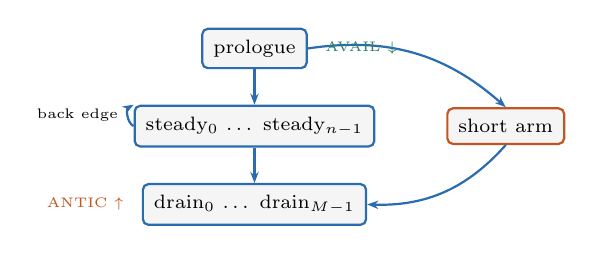
\begin{tikzpicture}[node distance=4.5mm,font=\scriptsize]
\node[box] (p) {prologue};
\node[box,below=of p] (s) {steady$_0$ \dots\ steady$_{n-1}$};
\node[box,below=of s] (d) {drain$_0$ \dots\ drain$_{M-1}$};
\node[wbox,right=9mm of s] (sh) {short arm};
\draw[ar] (p) -- (s); \draw[ar] (s) -- (d);
\draw[ar] (p.east) to[bend left=25] (sh.north);
\draw[ar] (sh.south) to[bend left=25] (d.east);
\draw[ar] (s.west) to[bend left=60] node[left,font=\tiny]{back edge} (s.north west);
\node[right=1mm of p,font=\tiny,text=ok] {AVAIL $\downarrow$};
\node[left=1mm of d,font=\tiny,text=warn] {ANTIC $\uparrow$};
\end{tikzpicture}
\end{column}
\end{columns}
\vspace{1mm}
\footnotesize
\key{Formulation:} a requirement is a value demanded at a point; a swap / increment is a \emph{definition} of
that value; ``where do defs go'' is classical code motion --- forward \textbf{AVAIL} $\times$ backward
\textbf{ANTIC}, a def wherever supply meets a different demand. Crossing $p\!\to\!b$ re-expresses the value via
\texttt{edge\_delta(p,b)}, so a drain value and a steady value are never compared as raw integers.
\good{Three pointers (LDS read, TDM descriptor, global-read address) share one 250-line solver; both
\texttt{on\_conflict} callbacks \emph{raise} --- report, never resolve.}
\end{frame}

% ==== frames/060_03.tex
\begin{frame}{A token names a SET of generations --- that is exactly what makes a loop-carried dependence visible to a backend that only sees an order}
\footnotesize
A memory token is not a label: it is an \key{LDS pseudo-register}. Downstream, a copy \emph{defs} it, a read
\emph{uses} it, a barrier does \emph{both} --- and ordinary def-use machinery does the rest. The token relation is
an alias relation and nothing else.

\begin{center}
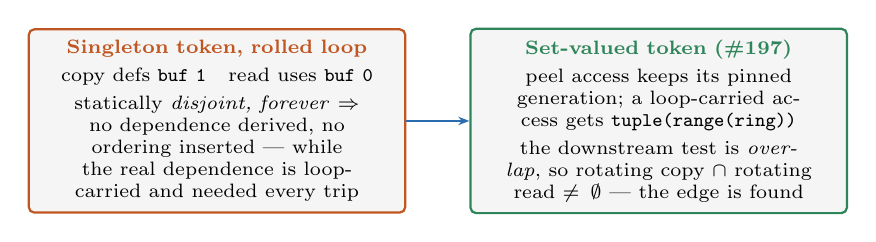
\begin{tikzpicture}[font=\scriptsize,node distance=4mm]
\node[wbox,text width=4.5cm] (n) {\bad{Singleton token, rolled loop}\\[2pt]
 copy defs \texttt{buf 1}\quad read uses \texttt{buf 0}\\[2pt]
 statically \emph{disjoint, forever} $\Rightarrow$ no dependence derived, no ordering inserted ---
 while the real dependence is loop-carried and needed every trip};
\node[gbox,right=8mm of n,text width=4.5cm] (w) {\good{Set-valued token (\#197)}\\[2pt]
 peel access keeps its pinned generation; a loop-carried access gets \texttt{tuple(range(ring))}\\[2pt]
 the downstream test is \emph{overlap}, so rotating copy $\cap$ rotating read $\neq\emptyset$ --- the edge is found};
\draw[ar] (n) -- (w);
\end{tikzpicture}
\end{center}

\begin{columns}[T]
\begin{column}{0.5\textwidth}
\textbf{The asymmetry that governs every choice here}
\begin{center}\scriptsize
\begin{tabular}{@{}ll@{}}
\toprule
token too \bad{narrow} & a miscompile \\
token too \good{wide} & a redundant wait, never wrong \\
\bottomrule
\end{tabular}
\end{center}
So every deliberate imprecision is a \emph{widening}.
\end{column}
\begin{column}{0.5\textwidth}
\textbf{And then the set was retired (\#207)}\\[2pt]
A set is a \emph{may}-set on a channel written for a \emph{must}-set --- and it says \emph{that} two
instructions collide, not \emph{after how many trips}. Once GIR derived the hazard edges itself and stood a
\key{fence} between the ends, the fence carries the must-set and receives each token as def \emph{and} use, so
\texttt{copy $\to$ fence $\to$ read} chains directly. Tokens went back to naming one buffer.
\end{column}
\end{columns}
\end{frame}

% ==== frames/060_07.tex
\begin{frame}{An LDS hazard is a trip distance --- and exactly one bit of it is load-bearing}
\footnotesize
\begin{columns}[T]
\begin{column}{0.5\textwidth}
An access carries offset $g$ (\texttt{gdelta}) on a ring of depth $S$; the back edge advances by \texttt{adv}:
\[ \mathrm{buf}(v,g) = (\text{base} + v\!\cdot\!\mathrm{adv} + g) \bmod S \]
Two accesses collide when
\[ (v_c - v_p)\cdot \mathrm{adv} \equiv (g_p - g_c) \pmod S \]
and with $\mathrm{adv}=1$ (every kernel today) the \key{trip distance} is
\[ d = (g_p - g_c) \bmod S \]
\good{The base cancels} --- so no absolute buffer identity is needed, which is fortunate, because in the one place
it would be needed it provably does not exist. Deriving $d$ from resolved generations instead would compare
\emph{representative-trip} values and under-report every pair that agrees on a different trip.
\end{column}
\begin{column}{0.5\textwidth}
\begin{center}\scriptsize
\begin{tabular}{@{}lll@{}}
\toprule
family & dir. & what breaks without ordering \\
\midrule
RAW \tsub{residency} & w$\to$r & read sees stale data \\
WAR \tsub{rotation} & r$\to$w & copy overwrites unread buffer \\
WAW \tsub{rotation} & w$\to$w & two copies, unconstrained order \\
\bottomrule
\end{tabular}
\end{center}
\vspace{2pt}
\textbf{The one bit:} \texttt{same\_trip} $\equiv (d=0)$.
$d=0$ $\Rightarrow$ discharge \emph{inside} the body, between the two accesses (an \emph{interval} of admissible
slots). $d\neq0$ $\Rightarrow$ purely loop-carried, so any fence in the body is crossed on the way --- a
\emph{union of two} intervals. \key{That union is why fence placement is a set cover and not a shortest-interval
problem.}\\[3pt]
\tsub{Two independent derivations agree: TensileLite's barrier pass skips at \texttt{numWaves == 1}; this analysis
reads only per-op-class agent distribution and finds 84 hazards on each of three single-wave fixtures, of which
\textbf{zero} need a fence.}
\end{column}
\end{columns}
\vspace{1mm}
\bad{Why the back end cannot do this:} its phase machine walks a flat stream keyed on a static label. It cannot see
a dependence whose producer and consumer are the \emph{same static instruction on two different trips} --- which,
in a rolled loop, is every loop-carried LDS dependence.
\end{frame}

% ==== frames/090_04.tex
\begin{frame}{One barrier per obligation was not a worse analysis --- it was an unbatched one}
\begin{center}
{\scriptsize
\begin{tabular}{llll}
\toprule
\textbf{formulation} & \textbf{problem shape} & \textbf{result} & \textbf{verdict} \\
\midrule
one fence per obligation & --- & \bad{28--48} barriers; the back end needs 7--10 & the baseline \\
interval greedy & interval cover & splitting a union over-fences & \bad{wrong}, not just larger \\
ILP / exact search & set cover & microseconds at this size & unstable tie-breaks \\
greedy cover & set cover & \good{6 fences for 1284 cross-agent edges} & shipped \\
\bottomrule
\end{tabular}}
\end{center}
\vspace{2mm}
\begin{itemize}
\item A fence is a \key{cover}, not the realization of an obligation: one point discharges every
      edge it happens to stand between. Only cross-agent edges need one, so a single-wave kernel
      gets \good{zero} --- independently agreeing with the back end's own one-wave skip.
\item A loop-carried pair's admissible slots are $\{s>a\}\cup\{s\le b\}$ --- a \key{union wrapping
      the body}, not an interval. That one fact forces set cover.
\item The \emph{points} are minimised; the \emph{names on each point} are not --- token
      permeability, from chapter 6, is what forbids minimising both.
\item ILP was rejected on determinism, not cost --- solver tie-breaking would make the emitted
      assembly non-reproducible.
\end{itemize}
\end{frame}

\section{Passes, verification, emission}
% ==== frames/070_01.tex

\begin{frame}{The pass order is not a preference: every adjacent pair is fixed by a dependency}
\centering
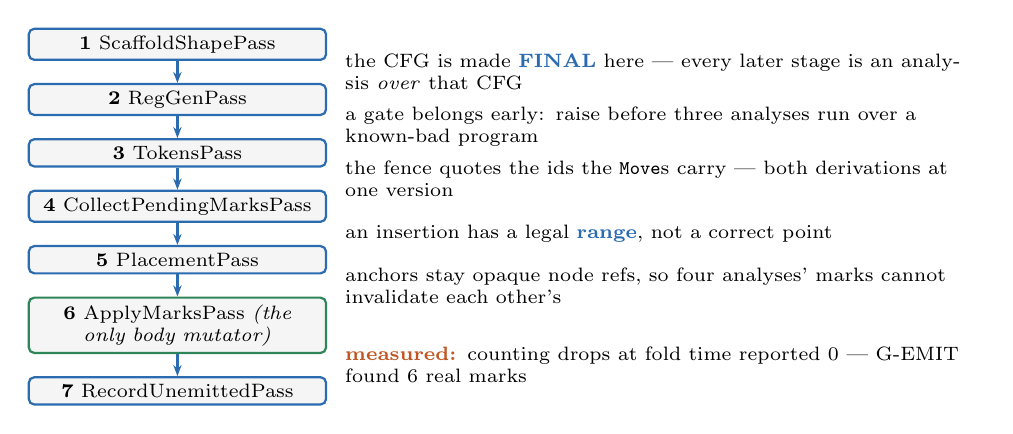
\begin{tikzpicture}[node distance=0.28cm, every node/.style={font=\scriptsize}]
\node[box,inner sep=2.5pt,text width=3.6cm] (p1) {\textbf{1} ScaffoldShapePass};
\node[box,inner sep=2.5pt,text width=3.6cm,below=of p1] (p2) {\textbf{2} RegGenPass};
\node[box,inner sep=2.5pt,text width=3.6cm,below=of p2] (p3) {\textbf{3} TokensPass};
\node[box,inner sep=2.5pt,text width=3.6cm,below=of p3] (p4) {\textbf{4} CollectPendingMarksPass};
\node[box,inner sep=2.5pt,text width=3.6cm,below=of p4] (p5) {\textbf{5} PlacementPass};
\node[gbox,inner sep=2.5pt,text width=3.6cm,below=of p5] (p6) {\textbf{6} ApplyMarksPass \emph{(the only body mutator)}};
\node[box,inner sep=2.5pt,text width=3.6cm,below=of p6] (p7) {\textbf{7} RecordUnemittedPass};

\draw[ar] (p1)--(p2) node[midway,anchor=west,xshift=2.0cm,text width=8.0cm,align=left]
  {the CFG is made \key{FINAL} here --- every later stage is an analysis \emph{over} that CFG};
\draw[ar] (p2)--(p3) node[midway,anchor=west,xshift=2.0cm,text width=8.0cm,align=left]
  {a gate belongs early: raise before three analyses run over a known-bad program};
\draw[ar] (p3)--(p4) node[midway,anchor=west,xshift=2.0cm,text width=8.0cm,align=left]
  {the fence quotes the ids the \texttt{Move}s carry --- both derivations at one version};
\draw[ar] (p4)--(p5) node[midway,anchor=west,xshift=2.0cm,text width=8.0cm,align=left]
  {an insertion has a legal \key{range}, not a correct point};
\draw[ar] (p5)--(p6) node[midway,anchor=west,xshift=2.0cm,text width=8.0cm,align=left]
  {anchors stay opaque node refs, so four analyses' marks cannot invalidate each other's};
\draw[ar] (p6)--(p7) node[midway,anchor=west,xshift=2.0cm,text width=8.0cm,align=left]
  {\bad{measured:} counting drops at fold time reported 0 --- G-EMIT found 6 real marks};
\end{tikzpicture}

\vspace{3pt}
{\scriptsize Then two gates: \texttt{verify\_gir} (twelve G-* checks) and
\texttt{\_check\_rotation\_waw}, the one invariant only true of a \emph{finished} program.}
\end{frame}

% ==== frames/070_03.tex
\begin{frame}{A checker that reports clean because it could not tell is worse than no checker}
\scriptsize
Two checkers, disjoint failure modes: \texttt{verify\_gir} asks \emph{is this IR well-formed?} (raises
on the first violation); \texttt{check\_plan} asks \emph{does this schedule compute the right GEMM?}
over the flat emit plan (returns a list). Neither subsumes the other.

\vspace{2pt}
\begin{tabular}{@{}l p{4.9cm} p{5.1cm}@{}}
\toprule
& \textbf{what it proves} & \textbf{how it can still pass} \bad{(named in the source)} \\
\midrule
G-TERM   & \texttt{preds}/\texttt{succs} agree with the terminators & an \emph{empty} tuple is never checked --- opt-in per block \\
G-CFG    & exactly $M$ drains; 0 \emph{or} exactly $M$ short blocks, agreeing with the verdict & \texttt{meta['M']} absent disables the count entirely \\
G-WALK   & the region walk closes \emph{and} every copy is on the region the descriptor is on & a block with no split copies is trivially clean \\
G-TOKEN  & disjoint LDS storage never shares an id; the \key{stamp} matches the analysis & the fence cover is checked non-empty, never \emph{sufficient} \\
G-EMIT   & marks dropped into blocks nobody emits are counted & compares a count, not the kind multiset \\
G-UNIFORM & a proc-scoped rendezvous is on every agent's path & \bad{structurally inert:} \texttt{role} is \texttt{'all'} everywhere and \texttt{Pred} cannot spell an agent test \\
\bottomrule
\end{tabular}

\vspace{3pt}
\good{The guard:} every check needs a negative control --- a fixture that breaks the property and
asserts the checker fires. \texttt{walk\_violations} first checked only the \emph{net} displacement;
hoisting every increment mark to the block entry leaves the net at zero while every copy loads the
wrong region. Net-clean and uniformly wrong. Its control now parameterises over
\texttt{drop}/\texttt{duplicate}/\texttt{hoist}.
\end{frame}

% ==== frames/080_05.tex
\begin{frame}{A model is verified only when a \emph{second, independently derived} implementation agrees}

\begin{columns}[T]
\begin{column}{0.50\textwidth}
\footnotesize
The LDS address is not computed by \texttt{LraTileAssignment} --- it is \emph{emitted} by it. Two
ways to check it:

\smallskip
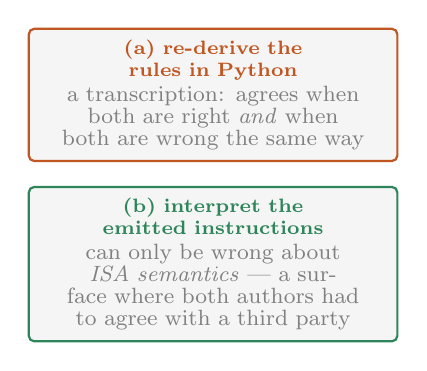
\begin{tikzpicture}[font=\scriptsize,node distance=3mm]
\node[wbox,text width=44mm] (a) {\bad{(a) re-derive the rules in Python}\\[1pt]
  \tsub{a transcription: agrees when both are right \emph{and} when both are wrong the same way}};
\node[gbox,below=of a,text width=44mm] (b) {\good{(b) interpret the emitted instructions}\\[1pt]
  \tsub{can only be wrong about \emph{ISA semantics} --- a surface where both authors had to agree
  with a third party}};
\end{tikzpicture}

\smallskip
\key{\texttt{asm\_lane\_eval.LaneEval}} executes a straight-line slice of gfx1250 asm once per
lane (32 lanes, Wave32) and reports per-lane register values. \texttt{lds\_region\_check} then
divides each address by the writer's \emph{own} split boundary and asks: does one
\texttt{ds\_load} touch two regions?

\smallskip
Two distinct faults: \bad{within-wave} straddle --- \emph{unrepresentable}, no coordinate fixes
it; \bad{across-wave} --- representable, but a race if the model was not told.
\end{column}

\begin{column}{0.48\textwidth}
\footnotesize
\textbf{Refusal is the design}

Any opcode or operand it cannot model raises \texttt{UnsupportedInstruction}. A silently-skipped
instruction leaves a stale register, and the address then \emph{looks like an address}.

\smallskip
\begin{tabular}{@{}p{0.95\textwidth}@{}}
\toprule
The first version returned \texttt{0} for an unwritten VGPR, reasoning that a backward slice is
closed under its own producers. \bad{It is not} --- it bottoms out at kernel \emph{inputs}. Every
address register then evaluated to exactly its \texttt{offset:} immediate, all lanes looked like
region~0, and the checker reported \bad{zero violations for four kernels}: a clean bill of health
produced entirely by reading uninitialised state. \\
\bottomrule
\end{tabular}

\medskip
\key{And the corollary: a differential oracle must first be shown \emph{capable of disagreeing} at
the input in question.} \texttt{region\_derivation\_check} recomputes the region from tile
\emph{position} vs tile \emph{index} --- it pinned the wave-span defect --- but it shares
\texttt{tiles\_per\_region}'s \texttt{max(1,\,.\,.\,)} floor, so at \texttt{MIWaveTile 1} both
derivations collapse to zero and it reports agreement it is \bad{incapable of withholding}.

\smallskip
\good{Add an oracle here, and add with it a test that makes the oracle fail.}
\end{column}
\end{columns}
\end{frame}

% ==== frames/070_06.tex
\begin{frame}{The leaf boundary decides HOW --- never WHAT, WHERE or WHY}
\centering
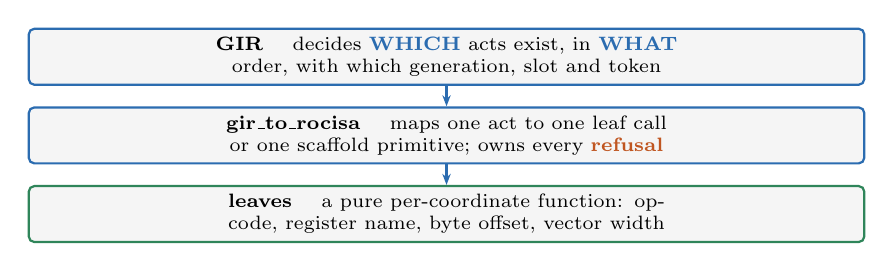
\begin{tikzpicture}[node distance=0.26cm, every node/.style={font=\scriptsize}]
\node[box,inner sep=3pt,text width=10.4cm] (a)
  {\textbf{GIR} \quad decides \key{WHICH} acts exist, in \key{WHAT} order, with which generation, slot and token};
\node[box,inner sep=3pt,text width=10.4cm,below=of a] (b)
  {\textbf{gir\_to\_rocisa} \quad maps one act to one leaf call or one scaffold primitive; owns every \bad{refusal}};
\node[gbox,inner sep=3pt,text width=10.4cm,below=of b] (c)
  {\textbf{leaves} \quad a pure per-coordinate function: opcode, register name, byte offset, vector width};
\draw[ar](a)--(b); \draw[ar](b)--(c);
\end{tikzpicture}

\vspace{4pt}
\scriptsize
\begin{itemize}\itemsep2pt
  \item \key{The claim that licenses it:} for a dense WMMA GEMM the machine code for one tile does
        not depend on the loop order at all. The schedule decides only which coordinates exist and
        in what sequence.
  \item \key{Nothing is re-derived.} Every fact arrives on the act or from a call into the active
        \texttt{KernelWriterAssembly}. Register names come from
        \texttt{generateSrcStrForMFMA}, accumulators from \texttt{accVgprReadWriteIndex} --- because
        re-spelling them here is a second derivation that agrees on the common case.
  \item \key{Refusals live in the adapter}, not in the leaves: six
        \texttt{NotImplementedError}s meaning \emph{GIR can express this, the scaffold cannot
        realize it}. A shape whose formula was never compared against the scaffold's own output is
        rejected by name, not generalized.
  \item \bad{The boundary is sharp and it has been crossed.} \texttt{Decision.reg\_slot} is the
        \emph{carrier} (the instruction ordinal), not the \emph{slot} (the position inside it).
        Feeding \texttt{slot} to the leaf renamed every scale register and failed all 16
        microscaling cells; the test that certified it had asserted the wrong one of the two.
  \item \tsub{Honest residue: \texttt{Decision.narrowed} is a socket nothing wires --- narrowing
        needs an instruction-selection choice the caller owns. Either wire it or delete it.}
\end{itemize}
\end{frame}

\section{Address geometry}
% ==== frames/080_01.tex

\begin{frame}{Two files import nothing --- and that emptiness is the feature}

\begin{columns}[T]
\begin{column}{0.46\textwidth}
\footnotesize
\key{\texttt{tdm\_split.py}} imports \texttt{dataclasses}. \\
\key{\texttt{lds\_geometry.py}} imports one name from \texttt{tdm\_split}. \\
No \texttt{Solution}, no \texttt{KernelWriter}, no \texttt{tP}, no rocisa.

\medskip
Functions needing more than three scalars take a \key{duck-typed context} --- so the
\emph{declaration} can live at the caller and the \emph{arithmetic} lives here.

\medskip
\good{Consequence:} \texttt{region\_row\_elems(32,0,False,2)} can be called in a bare
\texttt{pytest} and asserted \texttt{== 16}. The test it replaced had to match \emph{source
text}, and broke the moment the wrong expression was corrected.

\medskip
\bad{Do not add an import to either file.} Both docstrings state that obligation.
\end{column}

\begin{column}{0.52\textwidth}
\centering
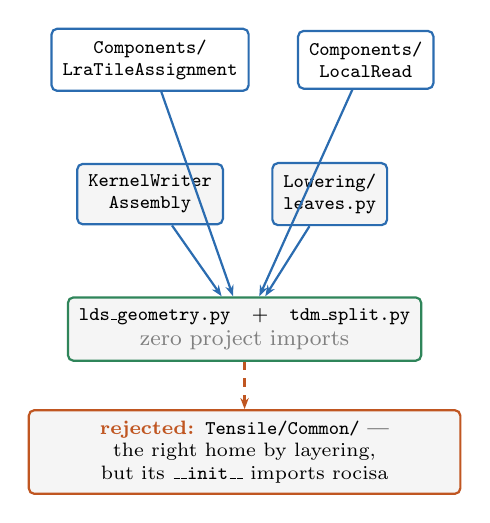
\begin{tikzpicture}[node distance=3mm,font=\scriptsize]
\node[box,fill=white] (lra) {\texttt{Components/}\\\texttt{LraTileAssignment}};
\node[box,fill=white,right=6mm of lra] (lr) {\texttt{Components/}\\\texttt{LocalRead}};
\node[box,below=9mm of lra] (kwa) {\texttt{KernelWriter}\\\texttt{Assembly}};
\node[box,right=6mm of kwa] (lv) {\texttt{Lowering/}\\\texttt{leaves.py}};
\node[gbox,below=9mm of kwa,xshift=12mm,minimum width=44mm]
   (geo) {\texttt{lds\_geometry.py} \; + \; \texttt{tdm\_split.py}\\[1pt]
          \tsub{zero project imports}};
\draw[ar] (lra) -- (geo);
\draw[ar] (lr) -- (geo);
\draw[ar] (kwa) -- (geo);
\draw[ar] (lv) -- (geo);
\node[wbox,below=6mm of geo,text width=52mm] (com)
   {\bad{rejected:} \texttt{Tensile/Common/} --- the right home by layering,
    but its \texttt{\_\_init\_\_} imports rocisa};
\draw[ar,draw=warn,dashed] (geo) -- (com);
\end{tikzpicture}

\smallskip
\footnotesize
Four emitters, three layers, \key{one derivation}. \texttt{Components/} reaches \emph{up} into
\texttt{Lowering/} on purpose. The one remaining option --- duplicating the formula --- is what
caused the defect two slides on.
\end{column}
\end{columns}
\end{frame}

\section{Evidence}
% ==== frames/010_03.tex
\begin{frame}{What shipped: the read trajectory, across the whole feature matrix --- and a named list of what is still absent}

{\scriptsize
\begin{tabular}{@{}llp{58mm}@{}}
\toprule
\textbf{Axis} & \textbf{Status} & \textbf{The measured number} \\
\midrule
bf16                  & \good{shipped}  & 5{,}744-kernel validation matrix \\
8-bit float           & \good{shipped}  & 152 kernels; 152/152 byte-identical emit-diff \\
MX-scaled fp8         & \good{shipped}  & 404--444 kernels; 404/404 byte-identical emit-diff, and 786 pass / 6 fail on the 792-cell hardware matrix \\
fp6 / fp4             & \bad{rejected}  & each has its own local-read packing; the read leaf's fragment table is checked against neither \\
Loop orders           & \good{shipped}  & six 3-letter words; 6-letter interleaved words require a split \\
Prefetch / look-ahead & \good{shipped}  & PGR sets the peel depth $M$; hard gate $S \ge$ PGR; PLR read-ahead is per register group \\
Tile split \tsub{(A/B)} & \good{shipped} & free-axis half; shared-K half only with no tail loop; mixed axes since 2026-08-18 \\
Multi-wave            & \good{shipped}  & $\Phi$ fuse: several movements, one cooperative instruction, \emph{one} completion \\
\bottomrule
\end{tabular}}

\vspace{2mm}
{\scriptsize \bad{Not covered, and each one is real work:} the epilogue and the whole write side
$\cdot$ the tail loop and the edge forks $\cdot$ wave specialization, whose two safety rules are
today \emph{structurally inert} $\cdot$ a persistent outer loop $\cdot$ register partitions $\cdot$
a second global-prefetch stage.}

\vspace{1mm}
{\scriptsize \key{The methodological lesson the numbers paid for:} the use-before-def gate was
written, correct, and called only from the unit tests. A later sweep flagged \key{216 of 216}
single-substep configurations. \emph{An oracle not on the build path is a test, not a gate.}}

\end{frame}

% ==== frames/090_08.tex
\begin{frame}{How it is validated: four layers, and each one is blind to something}
\begin{center}
{\scriptsize\setlength{\tabcolsep}{4pt}
\begin{tabular}{p{2.4cm}p{4.2cm}p{5.0cm}}
\toprule
\textbf{layer} & \textbf{what it proves} & \textbf{what it cannot catch} \\
\midrule
structural checks, on the build path &
schedule-gate properties, GIR well-formedness, and a per-kernel semantic check over the emit plan --- pure Python &
they read the structures the passes wrote, in the same vocabulary: good at inconsistency, \bad{blind to the model being uniformly wrong} \\
\addlinespace
fixtures and independent oracles &
22 named scenarios; a 168-cell order $\times$ split $\times$ prefetch sweep; simulators sharing \emph{no code} with what they check &
coverage bounded by whoever wrote the sweep. One check was correct, had four negative controls, and ran only from tests; a later sweep flagged \bad{216 of 216} single-substep cells and 0 of 432 elsewhere --- all sixteen hardware miscompares of that shape \\
\addlinespace
CPU-only generation, emit-diff vs.\ the old path &
\good{152 of 152} fp8 and \good{404 of 404} MX-scaled fp8 kernels byte-identical; both arms build locally &
byte equality proves you changed \emph{nothing}, so it is silent on any configuration the old path cannot generate; the coarse offset/count diff has missed two defect classes by ignoring registers and order \\
\addlinespace
hardware numerics &
the only layer that sees what the other three cannot &
it says \bad{wrong}, never \bad{where} --- one build cycle per bisection step \\
\bottomrule
\end{tabular}}
\end{center}
\begin{center}
\key{An oracle that is not on the build path is a test, not a gate.}
\end{center}
\end{frame}

% ==== frames/090_07.tex
\begin{frame}{What went wrong: two places computing one fact, agreeing on the common case}
\begin{center}
{\scriptsize\setlength{\tabcolsep}{4pt}
\begin{tabular}{lll}
\toprule
\textbf{the one fact} & \textbf{the two derivations} & \textbf{where they diverged} \\
\midrule
the region walk & the loader vs.\ the incrementer & $+2$ steps against $-1$: descriptor a chunk ahead \\
the rotation width & the scheduler's count vs.\ the name table & the degenerate in-place group \\
the token set & the analysis vs.\ the stamp on the move & a pass that truncated the stamp \\
the read-ahead depth & three different denominators & same on 100\% of the matrix, differing \\
 & & in \emph{form} on 47\% of it \\
the region a tile is in & the name it carries vs.\ where its lanes sit & agree at wave group [1,1], not at [2,2] \\
\bottomrule
\end{tabular}}
\end{center}
\vspace{1mm}
\begin{itemize}
\item \bad{A differential probe reporting ``no difference'' is worthless until it is shown able to
      report one.} The tile checker applies the same \texttt{max(1,\,$\cdot$)} floor as the
      derivation it checks: at one tile per two regions both collapse to region 0, so it is
      \emph{incapable} of disagreeing. A gate was removed on exactly that argument and the client
      \bad{segfaulted} --- 800 result rows before, 686 after. Reverted, with the argument preserved
      because it will be made again.
\item \bad{A rejection that only appears under the new path is a parity failure, not a safety
      feature} --- and a silent one: the solution stops appearing, its reference twin still passes,
      the matrix reads green with the arm under test absent. So the gate \key{raises}, and its
      contract is that it must never fire.
\end{itemize}
\end{frame}

\section{Where to go next}
% ==== frames/100_01.tex

\begin{frame}{Five known gaps, ranked --- and the first one is half a model}
\vspace{-2pt}
{\scriptsize
\begin{tabular}{@{}p{0.20\textwidth}p{0.30\textwidth}p{0.44\textwidth}@{}}
\toprule
\textbf{gap} & \textbf{what it blocks} & \textbf{what closing it takes} \\
\midrule
\key{1. the write / store side} &
the epilogue; the single-LDS-buffer configuration (the reuse is invisible to the hazard analysis); the ring-1 copy carries no WAR at all &
a movement whose destination is global space, a register-lifetime-vs-store hazard kind, an output operand with its own presence, a phase after the last drain --- plus reverse-pair counters and a reflected peel, which today \bad{refuses} rather than computes. \bad{Comparable in size to the read side.} \\
\addlinespace
\key{2. tail loop and edges} &
$K$ not a multiple of the chunk, free extents not a multiple of the tile: the old scaffold still serves them, so their reads and pointer state are outside the model &
a per-level peel for a \emph{runtime}-extent chunk. The hard half: drain and tail overlap under a reduction-axis storage split, and do not under a free-axis one \\
\addlinespace
\key{3. register partitioning} &
nothing --- and that is the problem: more than one group per operand is a \bad{silent no-op at emission} &
the per-\,(operand, group) widths are \good{already computed} and nothing reads them. Carry a per-group slot list in the emit plan, return the map instead of a scalar, teach the matrix leaf to select \\
\addlinespace
\key{4. half-wave scale selector} &
a fallback leaf re-derives a model-level fact: half the read acts stop issuing and the register index is compacted &
make the merge map \emph{derivable} rather than supplied. Four attempts to infer the pairing inside the model were each \bad{an address assumption in disguise} \\
\addlinespace
\key{5. persistent / grid-stride level} &
an outer time level above the reduction chunk &
one extra mode with extent 0 in $\theta$ --- no new level kind. What blocks it is the emitter refusing a coarser peel, and the frame arithmetic across an outer trip \\
\bottomrule
\end{tabular}}

\vspace{4pt}
{\footnotesize The tail's block phase exists, and the verifier already \emph{accepts} a tail as a second loop region. Nothing produces one. \bad{Expressible is not emitted} --- and each of these five is recorded in the source at the line that refuses.}
\end{frame}

% ==== frames/100_02.tex
\begin{frame}{Two packages, three optimisations worth doing --- and one bet}
\vspace{-2pt}
{\scriptsize
\begin{tabular}{@{}p{0.30\textwidth}p{0.64\textwidth}@{}}
\toprule
\texttt{Tensile/LoopModel/} & \key{the schedule model}: what happens \emph{when}. $\theta$, the peel, the ledger, the certificate. Every gate is either totality or honesty \\
\texttt{Tensile/Lowering/} & \key{the dataflow lowering}: \emph{where} each value lives. GIR, the analyses, the passes, the emitter. Each package carries its own gap list and cost map in-tree \\
\bottomrule
\end{tabular}}

\vspace{5pt}
{\footnotesize \key{Compile time}, measured not estimated: \good{8\,ms} of lowering on the common shape, \bad{165\,ms} on the worst measured one (4 waves, DepthU 512, a 1936-instruction body). Kernels build one per worker, so per-kernel wall time is what a sweep pays.}

\vspace{3pt}
{\scriptsize
\begin{tabular}{@{}p{0.52\textwidth}p{0.14\textwidth}p{0.12\textwidth}@{}}
\toprule
\textbf{ranked by win / risk} & \textbf{win} & \textbf{risk} \\
\midrule
fence slots as intervals + a difference array, not integer sets & $\sim$45\,ms & low \\
let the verifier accept the caller's analysis manager & $\sim$14\,ms & very low \\
hand the precomputed plan to the semantic gate & $\sim$12\,ms & none \\
\bottomrule
\end{tabular}}

\vspace{3pt}
{\footnotesize Everything below those is single-digit milliseconds. The CFG walks, the fixpoints and the token machinery are \emph{deliberately} not on the list --- they are free and they are the clearest code in the tree.}

\vspace{6pt}
\begin{center}
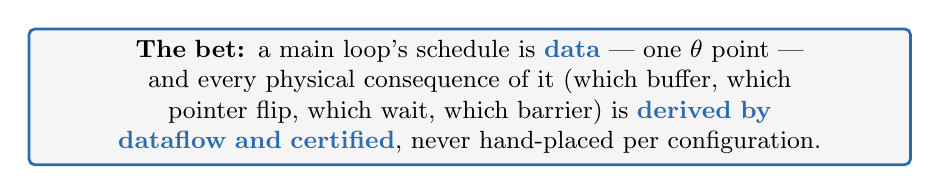
\begin{tikzpicture}
\node[box,draw=acc,line width=1pt,text width=0.90\textwidth,font=\small]{
\textbf{The bet:} a main loop's schedule is \key{data} --- one $\theta$ point --- and every physical
consequence of it (which buffer, which pointer flip, which wait, which barrier) is \key{derived by
dataflow and certified}, never hand-placed per configuration.};
\end{tikzpicture}
\end{center}
\end{frame}

\appendix
\section{Backup -- the schedule model}
% ==== frames/020_04.tex
\begin{frame}{What subtraction cost: a register ring rotating on a variable no loop binds}
\begin{center}
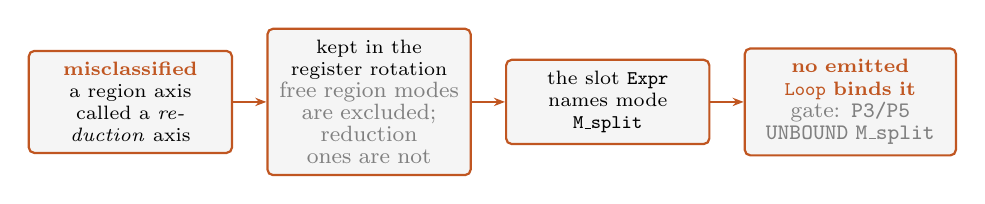
\begin{tikzpicture}[font=\scriptsize,node distance=6pt]
\node[wbox,text width=2.3cm] (a) {\bad{misclassified}\\a region axis called a \emph{reduction} axis};
\node[wbox,right=12pt of a,text width=2.3cm] (b) {kept in the register rotation\\\tsub{free region modes are excluded; reduction ones are not}};
\node[wbox,right=12pt of b,text width=2.3cm] (c) {the slot \texttt{Expr} names mode \texttt{M\_split}};
\node[wbox,right=12pt of c,text width=2.4cm] (d) {\bad{no emitted \texttt{Loop} binds it}\\\tsub{gate: \texttt{P3/P5 UNBOUND M\_split}}};
\draw[ar,draw=warn] (a)--(b); \draw[ar,draw=warn] (b)--(c); \draw[ar,draw=warn] (c)--(d);
\end{tikzpicture}
\end{center}
\vspace{-2pt}
\begin{itemize}\itemsep2pt
\item Each wave sees exactly \emph{one} value of that axis, so nothing in the read/compute nest
      rotates over it: the ring had a period nothing advanced.
\item \bad{Neither the ring, the gate, nor the slot expression was wrong.} All three did what they
      were told. The fault was a classification with no name for what the axis actually was.
\end{itemize}
\vspace{2pt}
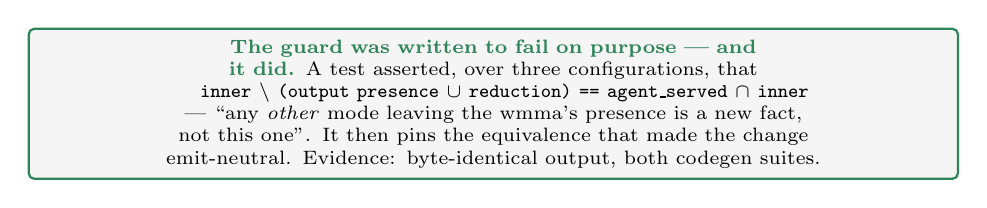
\begin{tikzpicture}
\node[gbox,text width=0.95\textwidth]{\good{The guard was written to fail on purpose --- and it did.}
A test asserted, over three configurations, that\\
\hspace*{1em}\texttt{inner \textbackslash{} (output presence $\cup$ reduction) == agent\_served $\cap$ inner}\\
--- ``any \emph{other} mode leaving the wmma's presence is a new fact, not this one''. It then pins
the equivalence that made the change emit-neutral. Evidence: byte-identical output, both codegen suites.};
\end{tikzpicture}
\end{frame}

% ==== frames/020_06.tex
\begin{frame}[fragile]{Retime is non-negative by type: deferral is a \emph{positive} offset on a reverse hop}
\begin{center}
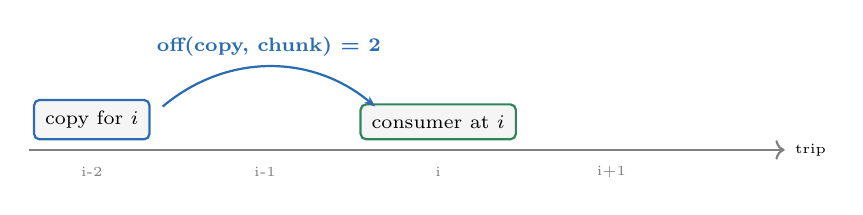
\begin{tikzpicture}[font=\scriptsize]
\draw[->,thick,draw=gray] (0,0) -- (9.6,0) node[right,font=\tiny]{trip};
\foreach \x/\l in {0.8/i-2,3.0/i-1,5.2/i,7.4/i+1} \node[font=\tiny,text=gray] at (\x,-0.28) {\l};
\node[box,anchor=south] at (0.8,0.12) {copy for $i$};
\node[gbox,anchor=south] at (5.2,0.12) {consumer at $i$};
\draw[ar,draw=acc] (1.7,0.55) to[out=40,in=140] node[above,font=\scriptsize]{\key{off(copy, chunk) = 2}} (4.4,0.55);
\end{tikzpicture}
\end{center}
\vspace{-4pt}
\begin{columns}[T]
\begin{column}{0.52\textwidth}
\begin{lstlisting}[style=py]
def off_at(self, opname, role, level_name):
    name = opname if isinstance(opname, str) \
           else opname.name
    return int(self.off_map.get(
        (name, role, level_name), 0))
\end{lstlisting}
\begin{itemize}\itemsep1pt
\item \key{Absent means 0} --- that op-class is simply not pipelined at that level, so the
      matrix stays sparse and no point enumerates the full cross product.
\item Prefer \texttt{off\_of(op, hop, level)}: it takes the role \emph{off the hop}. Restating
      the role at a call site is how a copy's offset gets read under the read's key.
\end{itemize}
\end{column}
\begin{column}{0.46\textwidth}
Two entries exist on the shipping parameter path:
\begin{center}\scriptsize
\begin{tabular}{ll}
\toprule
\texttt{off(copy, chunk)} & global prefetch depth \\
\texttt{off(read, substep)} & local prefetch depth \\
\bottomrule
\end{tabular}
\end{center}
\vspace{3pt}
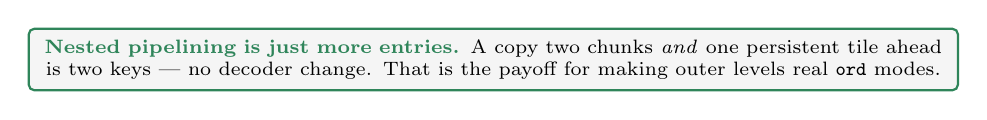
\begin{tikzpicture}
\node[gbox,text width=0.95\textwidth]{\good{Nested pipelining is just more entries.} A copy two chunks
\emph{and} one persistent tile ahead is two keys --- no decoder change. That is the
payoff for making outer levels real \texttt{ord} modes.};
\end{tikzpicture}
\vspace{2pt}

\bad{Nothing here enforces the sign.} A negative entry is rejected downstream, as ill-typed,
with that explanation.
\end{column}
\end{columns}
\end{frame}

\section{Backup -- placement}
% ==== frames/030_03.tex
\begin{frame}{Two structural vetoes cut the distance to zero --- at any width, for any $d$}

\textbf{Veto 1 --- the broadcast fan.} $\mathrm{fan}(p)$ = product of extents of the modes \emph{not} in
$\mathrm{pres}(p)$ that are outer, in \texttt{ord}, to \key{every} mode of $\mathrm{pres}(p)$. If the
whole name space is re-walked before any value dies, a hoisted write lands on a name a later consumer
still needs --- at \emph{any} distance. A race, not an anti-dependency.

\begin{columns}[T]
\begin{column}{0.56\textwidth}
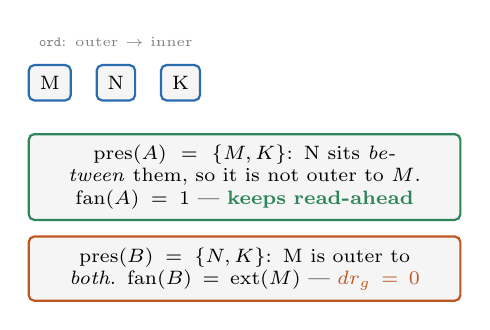
\begin{tikzpicture}[font=\scriptsize]
  \node[box] (m) {M};  \node[box,right=3mm of m] (n) {N};  \node[box,right=3mm of n] (k) {K};
  \node[font=\tiny,text=gray,above=1mm of n] {\texttt{ord}: outer $\rightarrow$ inner};
  \node[gbox,below=4mm of m.south west,anchor=north west,text width=52mm]
    {$\mathrm{pres}(A)=\{M,K\}$: N sits \emph{between} them, so it is not outer to $M$. $\mathrm{fan}(A)=1$ --- \good{keeps read-ahead}};
  \node[wbox,below=17mm of m.south west,anchor=north west,text width=52mm]
    {$\mathrm{pres}(B)=\{N,K\}$: M is outer to \emph{both}. $\mathrm{fan}(B)=\mathrm{ext}(M)$ --- \bad{$dr_g=0$}};
\end{tikzpicture}
\end{column}
\begin{column}{0.4\textwidth}
\begin{center}\scriptsize
\begin{tabular}{lcc}
\toprule
\texttt{ord} & $dr_g(A)$ & $dr_g(B)$ \\
\midrule
KMN, KNM & 1 & 1 \\
MNK, MKN & 1 & \bad{0} \\
NMK, NKM & \bad{0} & 1 \\
\bottomrule
\end{tabular}
\end{center}
\end{column}
\end{columns}

\vspace{1mm}
\textbf{Veto 2 --- a free sibling outer to the reduction.} The sibling is a storage-disjoint group, so
the shift cannot carry through it, \emph{and} the prologue's outer factor primes only region 0. Neither
half of the pipeline exists; in-place is the only consistent answer.

\tsub{Both vetoes live in the per-group derivation, not in the min that produces the steady advance --- a veto in the min alone zeroes the advance while the prologue keeps priming.}
\end{frame}

% ==== frames/030_05.tex
\begin{frame}[fragile]{The wrap lead has a closed form --- and prefetch-1 is degenerate, so three calibrated rules shipped wrong}

A staggered workgroup starts at chunk $S$, walks to $T-1$, then \key{wraps} to 0. The compare is
against the loop counter --- but the counter holds one value per trip, and the increments do not all
run in the trip whose number it holds. \texttt{lead} is that frame shift.

\begin{lstlisting}[style=pseudo]
prologue: increment #n targets chunk n, runs at ctr = T,  S = T-n => lead = pf - n
steady:   increment M+v+1,             runs at ctr = T-v, S = T-n => lead = pf - M - 1
                                          # v cancels: one instruction, all trips
          lead = pf - min(to_chunk, M + 1)
\end{lstlisting}

\begin{center}\scriptsize
\begin{tabular}{lccc}
\toprule
 & prologue, \texttt{to\_chunk}=1 & prologue, \texttt{to\_chunk}=2 & steady \\
\midrule
global prefetch 1 ($M{=}1$) & $+1$ & $0$ & \bad{$0$} \\
global prefetch 2 ($M{=}2$) & $+1$ & $0$ & \good{$-1$} \\
\bottomrule
\end{tabular}
\end{center}

At $M{=}1$ prologue and steady \bad{coincide at 0}, so any rule fitted there says nothing about
$M{=}2$. Three shipped in sequence --- $M-\texttt{to\_chunk}$; \texttt{1 if prologue};
\texttt{1 if to\_chunk==1} --- each passed its prefetch-1 tests, each gave the prefetch-2 steady
increment $0$ instead of $-1$: the wrap fires early, a whole tensor stride is subtracted, out of bounds.

\tsub{The same degeneracy bit \texttt{copy\_must\_be\_first} and the shared ring depth. Any rule over peel depth, prefetch depth or counter frame must be pinned against \emph{two} prefetch depths in one table. A negative lead is correct, not a sign error.}
\end{frame}

% ==== frames/030_07.tex
\begin{frame}{The degenerate arm is the unpipelined emission --- three displacements it must shed}

Not ``the steady body with knobs turned down''. A steady body assumes a \emph{predecessor trip}
supplied its opening producers; a fully-peeled level has neither predecessor nor prologue.

\begin{center}

\begin{tikzpicture}
\node[gbox,text width=92mm]{\textbf{Within the arm, every obligation's producer precedes its consumer.}};
\end{tikzpicture}
\end{center}

\begin{center}\scriptsize
\begin{tabular}{p{20mm}p{38mm}p{40mm}}
\toprule
displacement & mechanism & removed by \\
\midrule
\key{retime-carried} & the staggered copy ramp; the substep read-ahead & a copy phase with no ramp, and zero read shift --- a \emph{consequence} of emitting unpipelined, not the mechanism \\
\key{rotation-carried} & modulo-$S$ rotation writes each read after the matmul that vacates it; at $W{=}1$ this \bad{is} the only pipeline, and \bad{no retime value expresses it} & not applying the issue-order refinement, whose deferrals both order for a \emph{successor trip} the arm does not have \\
\key{order-carried} & the copy-first set derived from the \emph{steady} chunk crossing & re-deriving it: at zero retime a step's own copy is its true producer, so it must lead \\
\bottomrule
\end{tabular}
\end{center}

\tsub{Fixing one leaves the other two --- three separately diagnosed defects. The ledger caught none: a true-dependency obligation is generation-blind, so \texttt{await A@shared} was discharged by A's copy of chunk $t$ while the read wanted $t{+}1$. Empty ledger, passing gate, a buffer nothing had filled --- hence a structural test over the arm's own instructions.}
\end{frame}

\section{Backup -- obligations}
% ==== frames/040_02.tex
\begin{frame}{A closed vocabulary raises on a new kind; a suffix test \emph{schedules} it}

\begin{columns}[T]
\begin{column}{0.52\textwidth}
\vspace{-2pt}
\small
\begin{tabular}{@{}ll@{}}
\toprule
\multicolumn{2}{@{}l}{\texttt{RAW\_KINDS} --- true dependency} \\
\midrule
\texttt{RAW-residency} & consumer needs the moved value \\
\texttt{crossing-RAW}  & read-ahead reaches a chunk \emph{this} \\
                       & trip's own copy fills \\
\midrule
\multicolumn{2}{@{}l}{\texttt{WAR\_KINDS} --- anti-dependency} \\
\midrule
\texttt{rotation-WAR}  & refill writes a \emph{different} slot \\
\texttt{inplace-WAR}   & refill writes the \key{same} slot \\
\bottomrule
\end{tabular}
\vspace{6pt}

\texttt{OBLIGATION\_KINDS = RAW\_KINDS | WAR\_KINDS}, enumerated in exactly one place. \texttt{is\_war} is \key{total over a checked set} --- it raises rather than defaulting; \texttt{is\_raw} inherits the raise.
\end{column}
\begin{column}{0.46\textwidth}
\vspace{-2pt}
\bad{The prior form was \texttt{kind.endswith("WAR")} at eight sites.}

\vspace{4pt}
It fails in \emph{both} directions as soon as the vocabulary grows:
\begin{itemize}\itemsep2pt
  \item a new anti-dependency not spelled \texttt{...WAR} joins the RAW arm
  \item a true dependency that happens to end in those letters --- \texttt{read-after-WAR} --- joins the anti-dependency arm
\end{itemize}
Neither is an error. \bad{Both are a schedule} --- a slower kernel or a wrong answer, found on hardware.

\vspace{5pt}
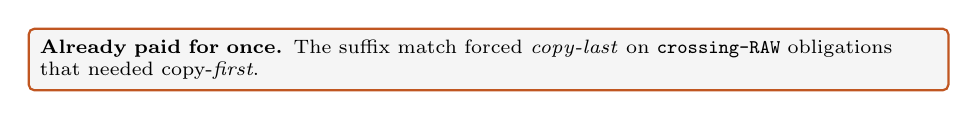
\begin{tikzpicture}
\node[wbox,text width=0.94\columnwidth,align=left] {\textbf{Already paid for once.} The suffix match forced \emph{copy-last} on \texttt{crossing-RAW} obligations that needed copy-\emph{first}.};
\end{tikzpicture}
\end{column}
\end{columns}
\end{frame}

% ==== frames/040_05.tex
\begin{frame}{Copies-last is \emph{scoped}, because at one setting the crossing read needs this trip's copy}

\begin{columns}[T]
\begin{column}{0.50\textwidth}
\vspace{-3pt}
One steady trip at chunk $c$ \key{reads} $c \ldots c{+}r$ and \key{writes} $c{+}\delta$, where $r$ is the read-ahead's chunk reach.

\vspace{3pt}
\small
\begin{tabular}{@{}lll@{}}
\toprule
relation & hazard & order \\
\midrule
$\delta = r$ ($r\ge1$) & \texttt{crossing-RAW} & copy \key{first} \\
$\delta \neq r$ & \texttt{*-WAR} or none & copy \key{last} \\
\bottomrule
\end{tabular}
\normalsize

\vspace{5pt}
Both shipping prefetch points sit at $S_{\text{shared}}{=}2,\ r{=}1$ and land on \emph{opposite} sides:
\begin{center}\ttfamily\scriptsize
depth 1: $\delta$=1, slot $(c{+}1)\bmod 2$ $\to$ hits the CROSSING read\\
depth 2: $\delta$=2, slot $c \bmod 2$\phantom{{+}1} $\to$ hits the CURRENT read
\end{center}

\vspace{3pt}
{\scriptsize \bad{An earlier predicate was $S_{\text{shared}} > r$} --- true for \emph{both}, so it emitted the depth-2 point copy-first and overwrote the buffer the trip was consuming.}
\end{column}
\begin{column}{0.47\textwidth}
\vspace{-3pt}
\textbf{The requirement} is scoped to $S_{\text{shared}} \le \delta$ --- there the refill is \key{in place} and the order is mandatory. Otherwise it is a rotation and the order is free. Both order checkers key on \texttt{inplace-WAR} \emph{alone}: \good{a \texttt{rotation-WAR} copy emitted first is not a violation.}

\vspace{5pt}
\textbf{The emitted policy is broader}: $\sigma_c$ defers \emph{both} WAR kinds unless vetoed --- ``last unless it must lead''.

\vspace{5pt}
\bad{The veto is only checkable because the RAW was modelled too.} With only the WAR present, nothing forced a copy to precede its own consumers --- correct at one chunk, wrong from two up.
\end{column}
\end{columns}
\end{frame}

% ==== frames/040_06.tex
\begin{frame}{A hazard analysis finds conflicts between things \emph{present}; absence is the schedule's job}

\begin{center}
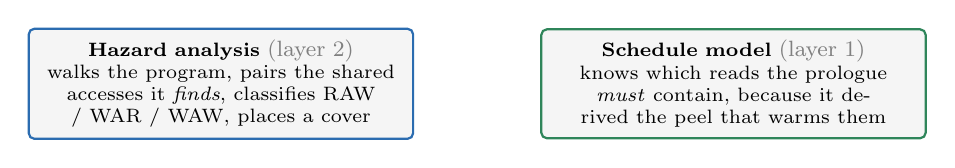
\begin{tikzpicture}[node distance=6mm]
\node[box,text width=4.6cm] (h) {\textbf{Hazard analysis} \tsub{(layer 2)}\\ walks the program, pairs the shared accesses it \emph{finds}, classifies RAW / WAR / WAW, places a cover};
\node[gbox,right=16mm of h,text width=4.6cm] (s) {\textbf{Schedule model} \tsub{(layer 1)}\\ knows which reads the prologue \emph{must} contain, because it derived the peel that warms them};
\end{tikzpicture}

\vspace{2pt}
{\footnotesize A read that was never emitted collides with nothing. It raises no pair, mints no edge, leaves no obligation undischarged.}
\end{center}

\vspace{-2pt}
\begin{columns}[T]
\begin{column}{0.49\textwidth}
\bad{Measured, twice.}
\begin{itemize}\itemsep2pt
  \item A drain read-ahead suppression window widened by one step: bf16 NT, $16{\times}16{\times}32$, $2{\times}2$ wave tile, \texttt{DepthU} 64 --- \key{62 \texttt{ds\_read}s at prefetch depths 1--2, 54 at depth 3}, against an unchanged 36 matmuls. Eight local reads gone, \bad{empty ledger, no warning}.
  \item The short-arm fold's \texttt{UNSOUND} verdict: an arm that reads a register it never wrote. Repaired for the data operands, \bad{never covered the microscaling scale operands}.
\end{itemize}
\end{column}
\begin{column}{0.49\textwidth}
\good{So existence is checked separately, and structurally.}
\begin{itemize}\itemsep2pt
  \item \texttt{readahead-residency} is an \emph{existence} obligation: arm (c) demands the coordinate be in the prologue body.
  \item Closed-form gates (\texttt{chunk\_crossing\_violations}) prune bad $(dr,\,\delta)$ pairs \emph{before} emission --- far better as a message: ``operand A, read-ahead 1, reach 1, depth 1, needs 2''.
\end{itemize}
\end{column}
\end{columns}
\end{frame}

\section{Backup -- the IR}
% ==== frames/050_04.tex
\begin{frame}{A hop is derived from the spaces, and a \texttt{Ref} names four residencies}
\centering
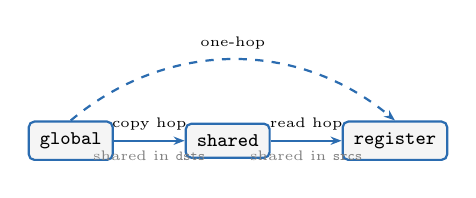
\begin{tikzpicture}[node distance=9mm,every node/.style={font=\scriptsize}]
  \node[box] (g) {\texttt{global}};
  \node[box,right=of g] (s) {\texttt{shared}};
  \node[box,right=of s] (r) {\texttt{register}};
  \draw[ar] (g) -- node[above,font=\tiny]{copy hop} node[below,font=\tiny,text=gray]{shared in \texttt{dsts}} (s);
  \draw[ar] (s) -- node[above,font=\tiny]{read hop} node[below,font=\tiny,text=gray]{shared in \texttt{srcs}} (r);
  \draw[ar,dashed] (g.north) to[out=40,in=140] node[above,font=\tiny]{one-hop} (r.north);
\end{tikzpicture}

\vspace{2pt}
{\scriptsize One \texttt{Move} class, no \texttt{Copy}/\texttt{Read} subclass --- so the analyses can walk
\emph{every} shared touch without a type switch, and "which movement is this?" is a
\bad{derived} property every new consumer must be told to get from \texttt{refs.py}.}

\vspace{5pt}
\begin{columns}[T]
\begin{column}{0.52\textwidth}
\scriptsize
\begin{tabular}{@{}ll@{}}
\toprule
\texttt{Ref} field group & residence \\
\midrule
\texttt{gen}, \texttt{gdelta}         & loop-carried shared \\
\texttt{abs\_gen}                     & pinned shared (peel, short arm) \\
\texttt{group}, \texttt{slot}, \texttt{reg\_ring} & register \\
\texttt{covers}                       & movement-quantum footprint \\
\bottomrule
\end{tabular}
\end{column}
\begin{column}{0.46\textwidth}
\scriptsize
\key{\texttt{gen} vs \texttt{abs\_gen}} is the peel/steady distinction made structural: a
prologue fill knows its buffer at compile time, a steady access does not.

\vspace{3pt}
\bad{"region" means two unrelated things} --- a \emph{storage} region (one piece of a split
LDS tile) and a \emph{placement} region (the legal window for a \texttt{Mark}).
They never share an expression, but they do share a file list.
\end{column}
\end{columns}
\end{frame}

% ==== frames/050_05.tex
\begin{frame}{An insertion has a legal \emph{range}, not a correct point}
\centering
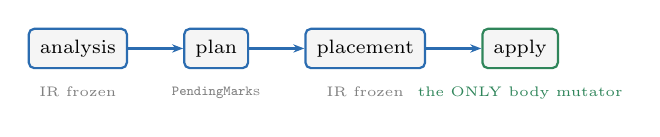
\begin{tikzpicture}[node distance=7mm,every node/.style={font=\scriptsize}]
  \node[box] (a) {analysis};
  \node[box,right=of a] (p) {plan};
  \node[box,right=of p] (l) {placement};
  \node[gbox,right=of l] (y) {apply};
  \draw[ar] (a) -- (p); \draw[ar] (p) -- (l); \draw[ar] (l) -- (y);
  \node[below=1mm of a,font=\tiny,text=gray] {IR frozen};
  \node[below=1mm of p,font=\tiny,text=gray] {\texttt{PendingMark}s};
  \node[below=1mm of l,font=\tiny,text=gray] {IR frozen};
  \node[below=1mm of y,font=\tiny,text=ok] {the ONLY body mutator};
\end{tikzpicture}

\vspace{6pt}
\begin{columns}[T]
\begin{column}{0.44\textwidth}
\centering
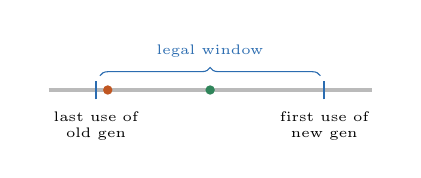
\begin{tikzpicture}[every node/.style={font=\tiny}]
  \draw[very thick,draw=lt!50!gray] (0,0) -- (4.1,0);
  \draw[thick,draw=acc] (0.6,-0.12) -- (0.6,0.12);
  \draw[thick,draw=acc] (3.5,-0.12) -- (3.5,0.12);
  \draw[decorate,decoration={brace,amplitude=3pt},draw=acc] (0.65,0.18) -- (3.45,0.18);
  \node[text=acc] at (2.05,0.5) {legal window};
  \node[anchor=north,text width=1.5cm,align=center] at (0.6,-0.15) {last use of\\old gen};
  \node[anchor=north,text width=1.5cm,align=center] at (3.5,-0.15) {first use of\\new gen};
  \node[circle,fill=warn,inner sep=1.2pt] at (0.75,0) {};
  \node[circle,fill=ok,inner sep=1.2pt] at (2.05,0) {};
  \node[text=warn,anchor=south] at (0.75,0.55) {};
\end{tikzpicture}
\vspace{1pt}

{\tiny \bad{$\bullet$ EARLIEST} descriptor edits \quad \good{$\bullet$ MIDPOINT} LDS read pointer}
\end{column}
\begin{column}{0.54\textwidth}
\begin{itemize}\scriptsize
  \item Anchors are \key{node references}, not indices --- a window survives other Marks
        landing in the same body before it resolves.
  \item Policy travels \emph{with} the region: a descriptor edit wants every cycle of overlap
        it can get; the read pointer is bounded by two different resources, so neither edge is right.
  \item Baking the index into the analysis is what the first version did --- and it is why
        placement policy could not be changed without rewriting the analysis.
\end{itemize}
\end{column}
\end{columns}

\vspace{3pt}
{\scriptsize One typed exception: \texttt{StructuralPass} may reshape the CFG. It exists because
\texttt{ApplyMarksPass} called itself "the only mutator" long after the fold pass had started
\bad{deleting blocks}. What is still \bad{unchecked}: two analyses placing conflicting Marks in one window.}
\end{frame}

% ==== frames/050_06.tex
\begin{frame}{The region is an AGENT fact on the read hop, a COORDINATE fact on the copy hop}
\centering
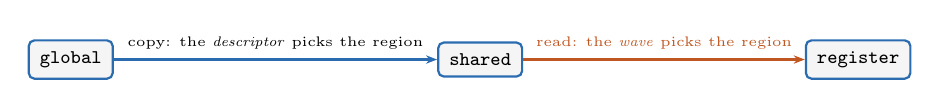
\begin{tikzpicture}[every node/.style={font=\scriptsize}]
  \node[box] (g) at (0,0) {\texttt{global}};
  \node[box] (s) at (5.2,0) {\texttt{shared}};
  \node[box] (r) at (10.0,0) {\texttt{register}};
  \draw[ar] (g) -- node[above,font=\tiny]{copy: the \emph{descriptor} picks the region} (s);
  \draw[ar,draw=warn] (s) -- node[above,font=\tiny,text=warn]{read: the \emph{wave} picks the region} (r);
\end{tikzpicture}

\vspace{4pt}
{\scriptsize A dump asserted, for a while: \bad{"wave $w$ reads region $w$, so one agent's reads name
one region."} Both halves false --- the block listing printed directly beneath it showed \texttt{A}
reading \emph{both} halves, and 8 of 8 agent-relative operands had disagreeing hops.}

\vspace{4pt}
\scriptsize
\begin{tabular}{@{}lp{7.3cm}@{}}
\toprule
consumer & what it does with the same one fact \\
\midrule
\texttt{mem\_tokens} (ordering) & \good{widen}: the read names \emph{every} region's token, or the producers it did not name go unordered \\
\texttt{check\_region\_coverage} & \good{narrow the demand}: under-coverage exempt (one agent never covers the set); over-coverage still faults --- a partition member cannot be a non-member \\
\texttt{render.py} (the dump) & print the per-hop split, and retract the sentence above \\
\bottomrule
\end{tabular}

\vspace{4pt}
{\scriptsize \bad{Three checkers each had to be taught this independently} --- one concept that
should have lived in one place. It also cost a day: a coverage message was read as proof the
\emph{model} needed a new narrowing construct, when the checker was asking a coordinate question
about an agent fact. \key{A violation message is evidence about the checker's premises too.}}
\end{frame}

\section{Backup -- the analyses}
% ==== frames/060_01.tex

\begin{frame}{A residence says three different things --- and the number every consumer wants is a fourth}
\begin{center}
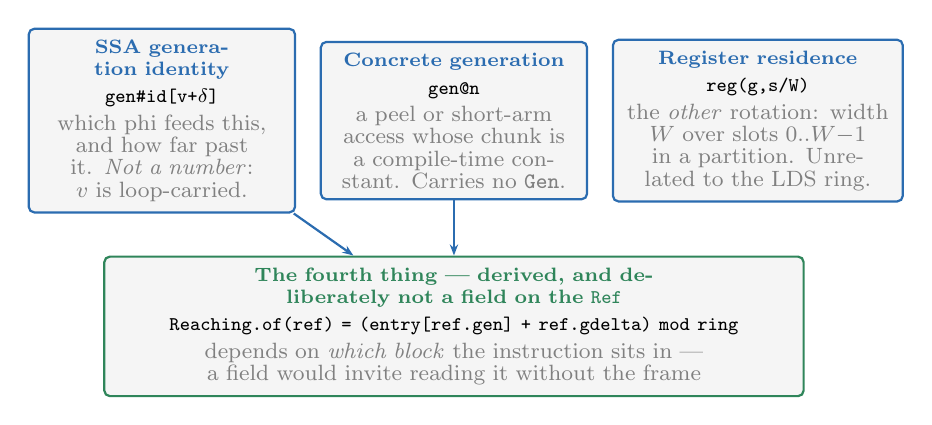
\begin{tikzpicture}[node distance=3mm]
\node[box,text width=3.1cm] (a) {\key{SSA generation identity}\\[2pt]
  \texttt{gen\#id[v+$\delta$]}\\[2pt]
  \tsub{which phi feeds this, and how far past it. \emph{Not a number}: $v$ is loop-carried.}};
\node[box,text width=3.1cm,right=of a] (b) {\key{Concrete generation}\\[2pt]
  \texttt{gen@n}\\[2pt]
  \tsub{a peel or short-arm access whose chunk is a compile-time constant. Carries no \texttt{Gen}.}};
\node[box,text width=3.4cm,right=of b] (c) {\key{Register residence}\\[2pt]
  \texttt{reg(g,s/W)}\\[2pt]
  \tsub{the \emph{other} rotation: width $W$ over slots $0..W{-}1$ in a partition. Unrelated to the LDS ring.}};
\node[gbox,below=7mm of b,text width=8.6cm] (d) {\good{The fourth thing --- derived, and deliberately not a field on the \texttt{Ref}}\\[2pt]
  \texttt{Reaching.of(ref) = (entry[ref.gen] + ref.gdelta) mod ring}\\[2pt]
  \tsub{depends on \emph{which block} the instruction sits in --- a field would invite reading it without the frame}};
\draw[ar] (a) -- (d); \draw[ar] (b) -- (d);
\end{tikzpicture}
\end{center}
\vspace{-1mm}
\footnotesize
\textbf{GenReaching} \quad domain: per block, \texttt{Gen $\to$ int}, a flat constant-propagation lattice \quad$\cdot$\quad
direction: forward \quad$\cdot$\quad
meet: \emph{agreement-or-bottom} (a \texttt{Gen} one predecessor supplies and another does not is \key{bottom}, not inherited).

\bad{The dump printed (1) as \texttt{gen0[v]} and (2) as \texttt{gen=0}} --- one character apart --- and chained the
three with early returns, so a register residence was invisible whenever a generation was present.
\end{frame}

% ==== frames/060_04.tex
\begin{frame}{If the token is not trip-invariant, the derived wait guards the wrong producer --- measured as \texttt{-nan}}
\footnotesize
\begin{center}
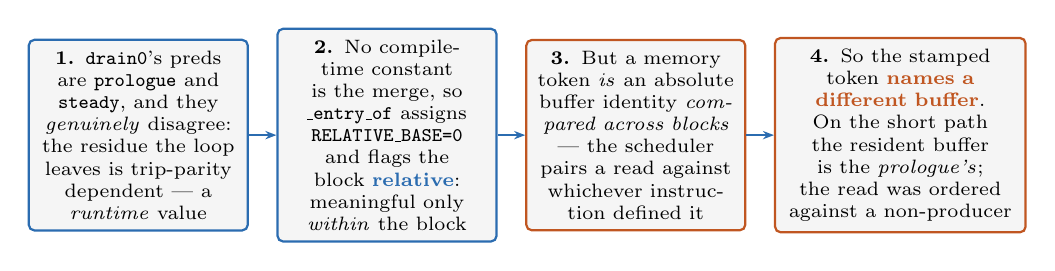
\begin{tikzpicture}[font=\scriptsize,node distance=3.5mm]
\node[box,text width=2.5cm] (s1) {\textbf{1.} \texttt{drain0}'s preds are \texttt{prologue} and \texttt{steady}, and they \emph{genuinely} disagree: the residue the loop leaves is trip-parity dependent --- a \emph{runtime} value};
\node[box,text width=2.5cm,right=of s1] (s2) {\textbf{2.} No compile-time constant is the merge, so \texttt{\_entry\_of} assigns \texttt{RELATIVE\_BASE=0} and flags the block \key{relative}: meaningful only \emph{within} the block};
\node[wbox,text width=2.5cm,right=of s2] (s3) {\textbf{3.} But a memory token \emph{is} an absolute buffer identity \emph{compared across blocks} --- the scheduler pairs a read against whichever instruction defined it};
\node[wbox,text width=2.9cm,right=of s3] (s4) {\textbf{4.} So the stamped token \bad{names a different buffer}. On the short path the resident buffer is the \emph{prologue's}; the read was ordered against a non-producer};
\draw[ar] (s1)--(s2); \draw[ar] (s2)--(s3); \draw[ar] (s3)--(s4);
\end{tikzpicture}
\end{center}

\begin{columns}[T]
\begin{column}{0.5\textwidth}
\bad{The measurement.} On a microscaling fp8 kernel: \texttt{-nan} in \textbf{23 of 540} swept cells,
\emph{every one on the short path}. A wrong-generation E8M0 scale poisons the multiply --- wrong-generation
\emph{data} often stays finite and silently wrong.\\[3pt]
\good{The fix, in the module's own idiom:} in a relative-frame block the access may touch \emph{every}
generation of the ring, so it carries every id. A redundant wait, where being optimistic loses one.
\end{column}
\begin{column}{0.5\textwidth}
\textbf{Two edges to keep:} an \texttt{abs\_gen} ref widens to \texttt{range(1)} --- correctly, it names a
concrete buffer whatever its block's phi frame does. And relativity must stay \key{transitive}: \texttt{drain1}'s
only predecessor is \texttt{drain0}, and ``one predecessor trivially agrees with itself'' once dropped the flag.\\[3pt]
\bad{Still open:} a \emph{legitimate} representative-trip frame read as invariant by a cross-trip consumer. Masked
in multi-wave (a fence stands between the ends anyway); single-wave has no fence, so the token is the only carrier.
\emph{Before narrowing a token, ask which consumer reads it.}
\end{column}
\end{columns}
\end{frame}

% ==== frames/060_05.tex
\begin{frame}{Barriers are PERMEABLE PER TOKEN --- so a fence must name everything live across it}
\footnotesize
A barrier is a \emph{point}, and its ordering power comes entirely from its token set: the downstream pass gives
it each token as both a def and a use. \bad{A buffer the barrier does not name is not chained through it at all}
--- accesses to it migrate across freely, and get no wait either.

\begin{center}
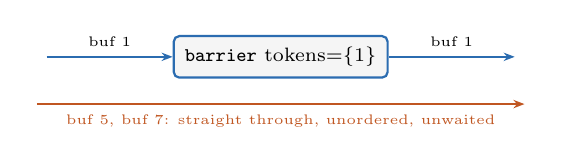
\begin{tikzpicture}[font=\scriptsize,node distance=6mm]
\node[box] (bar) {\texttt{barrier} tokens=$\{1\}$};
\node[left=16mm of bar] (l) {};
\node[right=16mm of bar] (r) {};
\draw[ar] (l) -- node[above,font=\tiny]{buf 1} (bar);
\draw[ar] (bar) -- node[above,font=\tiny]{buf 1} (r);
\draw[warn,thick,-{Stealth[length=4pt]}] ($(l)+(0,-6mm)$) -- node[below,font=\tiny,text=warn]{buf 5, buf 7: straight through, unordered, unwaited} ($(r)+(0,-6mm)$);
\end{tikzpicture}
\end{center}
\vspace{-2mm}
\begin{center}
\begin{minipage}{0.86\textwidth}
\key{The design rule that follows:} it does not get to be minimal in both dimensions.
The set of \textbf{POINTS} is minimised (a greedy set cover over admissible slots); the set of \textbf{NAMES}
on each point is \emph{not}.
\end{minipage}
\end{center}

\begin{columns}[T]
\begin{column}{0.52\textwidth}
\bad{The measurement that proved it.} A union-over-covered-edges fence was propped up by an unrelated
over-approximation. Fixing that widening shrank one steady fence's token list from $(1,5,7)$ to $(1,)$ and took a
multi-wave split configuration from 42 failures to \textbf{62}. The \emph{placement never moved} --- only the names
on it did. The widening had been doing liveness's job by accident for months.
\end{column}
\begin{column}{0.48\textwidth}
\begin{center}
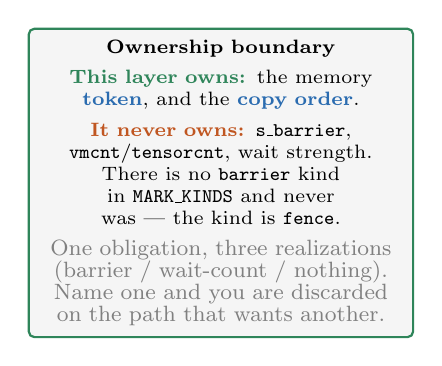
\begin{tikzpicture}[font=\scriptsize]
\node[gbox,text width=4.6cm] (o) {\textbf{Ownership boundary}\\[3pt]
 \good{This layer owns:} the memory \key{token}, and the \key{copy order}.\\[3pt]
 \bad{It never owns:} \texttt{s\_barrier}, \texttt{vmcnt}/\texttt{tensorcnt}, wait strength. There is no
 \texttt{barrier} kind in \texttt{MARK\_KINDS} and never was --- the kind is \texttt{fence}.\\[3pt]
 \tsub{One obligation, three realizations (barrier / wait-count / nothing). Name one and you are discarded on the
 path that wants another.}};
\end{tikzpicture}
\end{center}
\end{column}
\end{columns}
\end{frame}

% ==== frames/060_06.tex
\begin{frame}[fragile]{Existential reachability is not betweenness --- so ask the separation question directly}
\footnotesize
The cover is computed per block, so without a cross-block check it is blind: the last steady copy feeds reads in
\emph{two} drain blocks, and the second asks for a fence the first already provides.
``Is a fence in an earlier block already on every path?'' was approximated as:

\begin{center}\ttfamily\scriptsize
x in reachable(producer\_block) \quad and \quad x in dominators(consumer\_block) \quad\quad \bad{-- THE OLD FORM}
\end{center}

\bad{Why it is wrong:} \texttt{reachable} is \emph{existential} --- ``\emph{some} path from the producer reaches
$x$''. A candidate reachable only along a \key{back edge} satisfies it while sitting \emph{before} the producer on
every forward path. The hand-written \texttt{x != pb} guard was one instance of that general failure, seen once.

\begin{columns}[T]
\begin{column}{0.52\textwidth}
\begin{lstlisting}[style=pseudo]
_separates(x, pb, cb, succ):
  if pb == cb: return False
  stack = [s for s in succ[pb] if s != x]
  while stack:
    lab = pop(stack)
    if lab == cb: return False   # path avoids x
    if seen or lab == x: continue
    stack += [s for s in succ[lab] if s != x]
  return True                    # every path forced
\end{lstlisting}
\tsub{Starting at \texttt{pb}'s \emph{successors}, not at \texttt{pb}, is what makes a fence in the producer's own
block fail correctly.}
\end{column}
\begin{column}{0.48\textwidth}
\good{Delete $x$ from the graph. Is the consumer still reachable from the producer?} If not, every
producer$\to$consumer path is forced through $x$. One predicate subsumes reachability, dominance \emph{and} the
guard --- and needs no dominator tree.\\[4pt]
\textbf{Measured:} the old form left \bad{248 unfenced producer$\to$consumer paths in 14 of 36} swept
configurations, all \texttt{steady$_{n-1}$:copy $\to$ drain$_0$:read}, all at multi-block steady bodies.
The separator test drives \good{248 $\to$ 0} for \textbf{+1 fence} in 16 configurations --- and every
single-block-steady configuration, which is everything shipped today, is \good{bit-identical}.
\end{column}
\end{columns}
\end{frame}

% ==== frames/060_08.tex
\begin{frame}{One read \emph{act} is N instructions spaced by the LANE INTERLEAVE --- not by the per-thread input count}
\footnotesize
A read \texttt{Move} names one \texttt{(tile, reduction substep)} act. Layer 3 realizes it as N \texttt{ds\_read}s,
and both N and the \emph{spacing} are geometry GIR never sees. The natural guess --- ``this lane's elements are one
contiguous run'' --- is wrong in the spacing: consecutive chunks are \key{LANE\_INTERLEAVE} chunk-widths apart,
because the other lanes covering that K range each take a chunk in between.
\[ \mathrm{unrollElems}(i,v) = (v + i\cdot n_{\mathrm{in}}\cdot \mathrm{LANE\_INTERLEAVE})\cdot \mathrm{vwTrLoad}
\qquad \mathrm{LANE\_INTERLEAVE} = 2 = \tfrac{\mathrm{WavefrontSize}}{\mathrm{matrixInstTO}} \]
\vspace{-3mm}
\begin{columns}[T]
\begin{column}{0.54\textwidth}
\begin{center}\scriptsize
\begin{tabular}{@{}lrrrrrrr@{}}
\toprule
shape & bw & bpe & lrvw & ipt & miK & $n_{\mathrm{in}}$ & $n_{\mathrm{out}}$\\
\midrule
bf16 LDS-tr & 4 & 2 & 8 & 16 & 32 & 1 & 2\\
bf16 general & 4 & 2 & 8 & 16 & 32 & 1 & 2\\
fp8 LDS-tr & 2 & 1 & 16 & 32 & 64 & 2 & 2\\
\bad{fp8 general} & 4 & 1 & 16 & 64 & 128 & 1 & 4\\
\bottomrule
\end{tabular}
\end{center}
\tsub{Outer spacing $= n_{\mathrm{in}}\cdot\mathrm{LANE\_INTERLEAVE}\cdot\mathrm{vwTrLoad}$; the guess is
\texttt{inputPerThUnroll}. They agree only when the chunk count equals the interleave --- \emph{every} bf16 shape
and \emph{no} fp8 one.}
\end{column}
\begin{column}{0.46\textwidth}
\textbf{bf16:} $1\cdot2\cdot8 = 16$ vs \texttt{ipt} $=16$ --- identical. The wrong rule passed every test for as long
as bf16 was the only data type.\\[3pt]
\textbf{fp8 general:}
\begin{center}\ttfamily\scriptsize
\good{correct} ((0,0),(32,4),(64,8),(96,12))\\
\bad{guess\ \ } ((0,0),(64,4),(128,8),(192,12))
\end{center}
Three of four reads at the wrong K position. \bad{The registers still tile perfectly}, so a check that only
verified ``no gap, no overlap in registers'' waves the wrong table through. Hence two independent checks, and a
refusal rather than a plausible answer: \key{REGISTERS} \emph{and} \key{K EXTENT}
($n_{\mathrm{out}} n_{\mathrm{in}} \mathrm{vwTrLoad}\cdot\mathrm{LI} = \mathrm{MatrixInstK}$).
\end{column}
\end{columns}
\vspace{1mm}
\tsub{Consequence for hazards: \texttt{Access.pos} is a position among \emph{acts}, not instructions. A fence
between two acts is between all N fragments of each --- true for free, but only because a fence is never placed
\emph{inside} an act.}
\end{frame}

% ==== frames/060_09.tex
\begin{frame}{The short-path fold is a reordering-legality question --- and it is decided on VALUES reached, not producer identity}
\footnotesize
The degenerate ($T\le M$) path exists in every pipelined kernel. The scaffold serves it by \emph{skipping} the
loop; LoopIR emits a disjoint unpipelined arm. Folding deletes the arm and retargets the guard's false edge into
the drain head --- legal only if every def-use pairing survives the reordering
(\texttt{copy,compute,copy,compute} $\to$ \texttt{copy,copy $|$ compute,compute}).

\begin{columns}[T]
\begin{column}{0.5\textwidth}
\bad{Why producer identity gives confident false SPLITs.} The two arms are \emph{deliberately} different
schedules: the arm never enters the loop, so its read-ahead is reset ($dr=0$) while the drain keeps $dr(\theta)$.
They are not instruction-isomorphic, so ``same instruction'' is not a well-defined question.\\[3pt]
So each producer carries a value: a copy is \texttt{('copy',ops,coord,occurrence)} --- the $k$-th copy fetches
chunk $k$ on both arms --- and a read chains \key{transitively} to the copy that filled its buffer. Naming the
\emph{generation} instead identifies the chunk only while ring $\ge$ peel: at $S=1$ every generation is 0, a
false FOLD on exactly the configuration that needs the answer.\\[3pt]
\good{Under producer identity the shipping default reported 24 breaks --- every one an artefact.}
\end{column}
\begin{column}{0.5\textwidth}
\begin{center}\scriptsize
\begin{tabular}{@{}ll@{}}
\toprule
sweep & verdicts \\
\midrule
A: 6 orders $\times$ PGR 1--3 $\times$ PLR 0--1, $S{=}2$ & \textbf{24 FOLD / 12 SPLIT} \\
\quad \tsub{$M{=}1,2$ fold; $M{=}3$ splits, 8 \textsc{overwritten}} & \\
B: same shape forced to $S{=}1$ & $M{=}1$ folds; $M{=}2,3$ split \\
\quad \tsub{8 and 16 breaks, all \textsc{overwritten}} & \\
C: 22 named fixtures & \textbf{19 FOLD / 2 SPLIT / 1 NA} \\
\bottomrule
\end{tabular}
\end{center}
\tsub{Loop order does not enter the answer in any cell. The two C splits are \emph{not} ring-depth splits: 32 breaks
over 4 register locations, all \textsc{unwritten} --- the register-side warm-up gap.}\\[3pt]
\textbf{The summary is ``fold iff ring $\ge$ peel'' --- and the analysis deliberately does not test that
inequality.} It sees nothing of warm-up (an arm reading what it never wrote is \texttt{UNSOUND}, and the
inequality calls it foldable).\\[3pt]
\tsub{\good{The shipping default folds in all six orders} --- as it must, since the scaffold has done exactly
that for years.}
\end{column}
\end{columns}
\end{frame}

\section{Backup -- passes and emission}
% ==== frames/070_02.tex
\begin{frame}[fragile]{Adding a pass: the slot in the order is a claim you must justify}
\begin{columns}[T]
\begin{column}{0.50\textwidth}
\scriptsize
\textbf{1. Kind.} Are the block set, terminators and every
\texttt{preds}/\texttt{succs} identical on the way out? Yes $\to$ \texttt{Pass};
no $\to$ \texttt{StructuralPass}.

\textbf{2. Slot.}
\begin{itemize}\itemsep1pt
  \item touches the CFG $\to$ \key{inside ScaffoldShapePass}, never later
  \item produces \texttt{PendingMark}s $\to$ not a pass at all: an \key{Analysis} in
        \texttt{CollectPendingMarks}' list
  \item records a fact about the finished program $\to$ after \texttt{ApplyMarks}
\end{itemize}

\textbf{3. CFG changed $\to$ extend the verifier} (next slide).

\textbf{4. Test three ways:} standalone, through the pipeline, and a
\good{negative control} that builds the illegal shape.

\textbf{5.} Return what you invalidated --- and know that nobody reads it.
\bad{Rely on \texttt{prog.bump()}.}
\end{column}
\begin{column}{0.50\textwidth}
\begin{lstlisting}[style=py]
class MyPass(Pass):          # or StructuralPass
    """What it changes; WHY this slot."""
    def run(self, prog, am):
        f = am.get(SomeAnalysis(), prog)
        ...
        if changed:
            prog.bump()      # MANDATORY
        return ("invalidated",) if changed else ()
\end{lstlisting}
\scriptsize
Rules a reviewer looks for:
\begin{itemize}\itemsep1pt
  \item key on \texttt{Block.phase} or CFG shape, \bad{never a label}
  \item never re-derive a $\theta$ fact --- look it up in \texttt{prog.meta}
  \item rebuild \texttt{succs} with the terminator; recompute \texttt{preds} wholesale
  \item guard idempotence: tests run passes standalone
  \item \key{report, never resolve} --- raise naming every instance and the config
\end{itemize}
\end{column}
\end{columns}
\end{frame}

% ==== frames/070_04.tex
\begin{frame}{A pass that changes the CFG obliges the verifier to CHECK the new shape, not assume it}
\begin{columns}[T]
\begin{column}{0.40\textwidth}
\centering
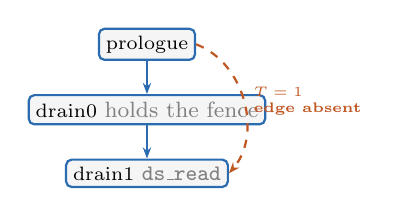
\begin{tikzpicture}[node distance=0.42cm, every node/.style={font=\scriptsize}]
\node[box,inner sep=2.5pt] (pro) {prologue};
\node[box,inner sep=2.5pt,below=of pro] (d0) {drain0 \tsub{holds the fence}};
\node[box,inner sep=2.5pt,below=of d0] (d1) {drain1 \tsub{\texttt{ds\_read}}};
\draw[ar] (pro)--(d0);
\draw[ar] (d0)--(d1);
\draw[-{Stealth[length=4pt]},thick,draw=warn,dashed]
  (pro.east) to[bend left=55] node[right,font=\tiny,text=warn,align=left]
  {$T=1$\\ \bad{edge absent}} (d1.east);
\end{tikzpicture}

\vspace{2pt}
\tsub{With the edge missing, \texttt{drain0} \emph{dominated} \texttt{drain1}, so the fence cover
elided \texttt{drain1}'s fence. True of the CFG it was given; false of the kernel.}
\end{column}
\begin{column}{0.58\textwidth}
\scriptsize
\bad{Measured:} 32 cross-agent hazard edges left unfenced; the microscaled-fp8 kernels returned
\texttt{-nan} on every $T \le M$ cell. The repair was structural --- all three CFG rewrites moved
into one stage that runs \key{first}, so ``the CFG is final before anything reasons over it'' is a
property of the pipeline's shape, not a convention.

\vspace{4pt}
The verifier side of the same rule:
\begin{itemize}\itemsep2pt
  \item \key{G-CFG} the fold may leave \good{0} short blocks (folded) or \good{exactly $M$} (kept)
        --- \bad{any other count} means a pass truncated the arm. Before the cross-check, silent
        truncation was indistinguishable from a correct fold.
  \item \key{G-EMIT} a block nobody emits must \emph{say so}, and its discarded marks must be counted.
  \item \key{G-TRIP} a pass that rotates the loop cannot quietly change the total work.
\end{itemize}

\vspace{3pt}
\tsub{Worked example --- a critical-edge splitter: \texttt{StructuralPass}, after the early exits,
before labelling. Its new block phased \texttt{"drain0.split"} would be \emph{counted as a drain} and
fail \texttt{n\_drain != M}. \texttt{phase} is a string doing type-system work.}
\end{column}
\end{columns}
\end{frame}

% ==== frames/070_05.tex
\begin{frame}{Load versus broadcast is DERIVED from the movement quantum, never declared}
\centering
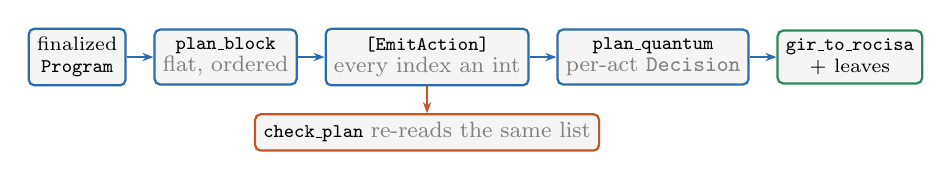
\begin{tikzpicture}[node distance=0.30cm and 0.34cm, every node/.style={font=\scriptsize}]
\node[box,inner sep=3pt] (prog) {finalized \\ \texttt{Program}};
\node[box,inner sep=3pt,right=of prog] (plan) {\texttt{plan\_block} \\ \tsub{flat, ordered}};
\node[box,inner sep=3pt,right=of plan] (acts) {\texttt{[EmitAction]} \\ \tsub{every index an int}};
\node[box,inner sep=3pt,right=of acts] (q) {\texttt{plan\_quantum} \\ \tsub{per-act \texttt{Decision}}};
\node[gbox,inner sep=3pt,right=of q] (rc) {\texttt{gir\_to\_rocisa} \\ + leaves};
\draw[ar](prog)--(plan); \draw[ar](plan)--(acts); \draw[ar](acts)--(q); \draw[ar](q)--(rc);
\node[wbox,inner sep=3pt,below=0.34cm of acts] (chk) {\texttt{check\_plan} \tsub{re-reads the same list}};
\draw[ar,draw=warn](acts)--(chk);
\end{tikzpicture}

\vspace{3pt}
\scriptsize
A quantum is the set of axes one movement \emph{instruction} covers, supplied from outside the model
as two index expressions over the tile coordinate. Nothing is tagged a broadcast:

\vspace{2pt}
\begin{tabular}{@{}l c c l@{}}
\toprule
mechanism & \texttt{carrier(t)} & \texttt{slot(t)} & \texttt{regs} \\
\midrule
wide load of 2 tiles & $t/2$ & $t \bmod 2$ & 2 --- each tile gets its own register \\
sub-agent broadcast, $N$ partitions & $(t/N)\cdot N$ & $0$ & 1 --- \key{partners SHARE a slot} \\
\bottomrule
\end{tabular}

\vspace{3pt}
The group is the \key{preimage} of \texttt{carrier}, not a contiguous run --- the sub-agent partner
sits a stride away. \bad{Measured:} a leaf that merged two acts on its own authority folded LDS
tokens 9 and 8 under one \texttt{ds\_load\_b64}; 4096 of 65536 outputs wrong. And
\texttt{WHOLE = None} is \emph{silence}, not a permissive decision: returning
\texttt{Decision(emit=True)} instead made the leaf skip its own fold and failed 16 of 16
microscaling cells, including the 10 that had been passing.
\end{frame}

\section{Backup -- address geometry}
% ==== frames/080_02.tex
\begin{frame}[fragile]{A partition packs blocks iff it cuts the image's \emph{inner} axis --- so the rule is a diagonal}

\begin{columns}[T]
\begin{column}{0.50\textwidth}
\footnotesize
LDS is linear, so the tile is serialised in one of two orders, chosen per operand by the
\key{memory layout} of the global tensor:

\smallskip
\begin{tabular}{@{}ll@{}}
\toprule
unroll-major & image \texttt{[free][unroll]} \\
tile-major   & image \texttt{[unroll][free]} \\
\bottomrule
\end{tabular}

\smallskip
The hardware writes each region \key{densely}. Cut the \emph{outer} axis and the regions are runs
of whole rows, adjacent --- the unsplit image is reproduced exactly. Cut the \emph{inner} axis and
a dense write cannot interleave stripes, so what lands is a different image.

\medskip
Stated once, in \texttt{tdm\_split.split\_packs\_lds}:

\begin{lstlisting}[style=py]
return (axis == AXIS_MT) == (not unrollMajor)
\end{lstlisting}
\tsub{an XNOR of "the cut is on the free axis" with "the free axis is inner"}
\end{column}

\begin{column}{0.48\textwidth}
\centering
\begin{tabular}{@{}lcc@{}}
\toprule
cut axis & unroll-major & tile-major \\
         & \tsub{[free][unroll]} & \tsub{[unroll][free]} \\
\midrule
\texttt{AXIS\_MT} \tsub{free}   & \good{contiguous} & \bad{PACKED} \\
\texttt{AXIS\_DU} \tsub{unroll} & \bad{PACKED}      & \good{contiguous} \\
\bottomrule
\end{tabular}

\medskip
\footnotesize
\key{Both cells of the MT row are measured --- one in the negative.}

\smallskip
\begin{tabular}{@{}p{0.94\textwidth}@{}}
\toprule
\bad{MT, tile-major $\rightarrow$ PACKED} (2026-08-17, NT MT32x32x64): without the packed
treatment every NT split kernel read region~0's bytes for half its tiles. \\
\midrule
\good{MT, unroll-major $\rightarrow$ CONTIGUOUS} (2026-08-16): \emph{adding} a region term here
regressed 82 passing kernels, 110 failures $\rightarrow$ 192. \\
\bottomrule
\end{tabular}

\smallskip
Same axis, two layouts, opposite treatment. \bad{Generalising either measurement to the other
layout is the defect.}
\end{column}
\end{columns}
\end{frame}

% ==== frames/080_03.tex
\begin{frame}{A packed split makes the address PIECEWISE --- and every consumer pays for it}

\centering
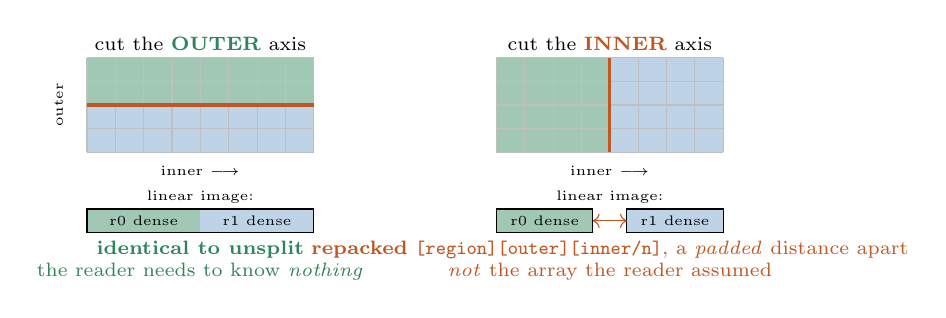
\begin{tikzpicture}[font=\tiny,x=3.6mm,y=3.0mm]
% ---- outer cut ----
\node[font=\scriptsize] at (4,4.6) {cut the \good{OUTER} axis};
\foreach \r in {0,1}{\foreach \c in {0,...,7}{\fill[ok!45] (\c,3-\r) rectangle ++(1,1);}}
\foreach \r in {2,3}{\foreach \c in {0,...,7}{\fill[acc!30] (\c,3-\r) rectangle ++(1,1);}}
\draw[step=1,gray!50,thin] (0,0) grid (8,4);
\draw[very thick,warn] (0,2) -- (8,2);
\node[font=\tiny,rotate=90] at (-1.0,2) {outer};
\node at (4,-0.8) {inner $\longrightarrow$};
\node at (4,-1.9) {linear image:};
\fill[ok!45] (0,-3.4) rectangle (4,-2.4); \fill[acc!30] (4,-3.4) rectangle (8,-2.4);
\draw (0,-3.4) rectangle (8,-2.4);
\node at (2,-2.9) {r0 dense}; \node at (6,-2.9) {r1 dense};
\node[align=center,font=\scriptsize,text=ok] at (4,-4.6)
  {\textbf{identical to unsplit}\\the reader needs to know \emph{nothing}};

% ---- inner cut ----
\begin{scope}[xshift=52mm]
\node[font=\scriptsize] at (4,4.6) {cut the \bad{INNER} axis};
\foreach \r in {0,...,3}{\foreach \c in {0,...,3}{\fill[ok!45] (\c,3-\r) rectangle ++(1,1);}}
\foreach \r in {0,...,3}{\foreach \c in {4,...,7}{\fill[acc!30] (\c,3-\r) rectangle ++(1,1);}}
\draw[step=1,gray!50,thin] (0,0) grid (8,4);
\draw[very thick,warn] (4,0) -- (4,4);
\node at (4,-0.8) {inner $\longrightarrow$};
\node at (4,-1.9) {linear image:};
\fill[ok!45] (0,-3.4) rectangle (3.4,-2.4); \fill[acc!30] (4.6,-3.4) rectangle (8,-2.4);
\draw (0,-3.4) rectangle (3.4,-2.4); \draw (4.6,-3.4) rectangle (8,-2.4);
\draw[<->,warn] (3.4,-2.9) -- (4.6,-2.9);
\node at (1.7,-2.9) {r0 dense}; \node at (6.3,-2.9) {r1 dense};
\node[align=center,font=\scriptsize,text=warn] at (4,-4.6)
  {\textbf{repacked} \texttt{[region][outer][inner/n]}, a \emph{padded} distance apart\\
   \emph{not} the array the reader assumed};
\end{scope}
\end{tikzpicture}

\vspace{2mm}
\raggedright\footnotesize
The packed reader owes \key{three} corrections, and they must all come off the \emph{same}
predicate: a per-region \key{block base}, a \key{shortened row} ($I/n + \text{pad}$), and an
\key{in-region inner coordinate} ($\text{inner} \bmod I/n$).

\smallskip
\bad{A division is unavoidable.} \texttt{region\,*\,splitBoundary} is a \emph{padded byte}
boundary, not an element stride, so the piecewise form has no linear expression. Any emitter that
accumulates (\texttt{rIdx*step + localReadOffset}) must divide --- \texttt{fold\_inner\_offset}
does it once so the scaffold path and the GIR path cannot disagree about where the boundary is.
Straddling reads are excluded by a \texttt{Solution.py} rejection, \texttt{(DepthU // n) \% MatrixInstK == 0}.
\end{frame}

% ==== frames/080_04.tex
\begin{frame}[fragile]{Every split failure traced to \emph{one} missing term in the tile stride --- not tokens, not waits}

\begin{columns}[T]
\begin{column}{0.53\textwidth}
\footnotesize
Turning splits on under GIR failed on hundreds of kernels, on both layouts, at several loop
orders. It had every characteristic of a \bad{synchronisation} bug: depth-dependent, changed with
prefetch, different at one wave vs four.

\smallskip
Memory tokens, derived waits, barrier placement, hop order --- \good{all of them were correct.}

\begin{lstlisting}[style=pseudo]
tile_row(t):
  was:  tileStrideElems * t
  is :  (t // VW) * MIWaveGroupShape + (t % VW)
\end{lstlisting}
\tsub{a wave takes VW adjacent rows, then jumps a whole group --- that jump is what hands the
intervening rows to the other waves}

\smallskip
Measured (MT32x32 KMN PGR2/PLR0, \emph{unsplit}), operand A \texttt{ds\_load} offsets:
\begin{lstlisting}[style=pseudo]
scaffold: 0,32,64,96, 2176,2208,2240,2272
ours    : 0,32,64,96,  128, 160, 192, 224
\end{lstlisting}
Wrong rows $\rightarrow$ sometimes the wrong \emph{region} $\rightarrow$ the \emph{correct} token
machinery then ordered a read against a producer that was not its producer. \key{The symptom
presented one layer above the defect.}
\end{column}

\begin{column}{0.45\textwidth}
\footnotesize
\textbf{Three reasons it stayed invisible}
\begin{enumerate}\itemsep1pt\parskip0pt
\item \bad{The wrong form is a special case of the right one.} At \texttt{MIWaveTile == VW} the
group term is zero --- and every fixture pinned \texttt{MIWaveTile == VW == 2}.
\item \bad{The failure was numeric, not structural.} \texttt{ds\_read offset:128} is as
well-formed as \texttt{offset:2176}.
\item \bad{The address is a sum of independently-chosen terms.} One wrong term still yields a
\emph{plausible} address --- right magnitude, alignment, region count.
\end{enumerate}

\smallskip
\centering
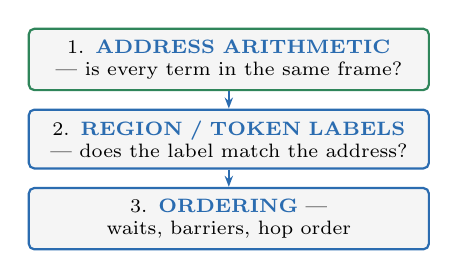
\begin{tikzpicture}[node distance=2.2mm,font=\scriptsize]
\node[gbox,text width=48mm] (a) {1. \key{ADDRESS ARITHMETIC} --- is every term in the same frame?};
\node[box,below=of a,text width=48mm] (b) {2. \key{REGION / TOKEN LABELS} --- does the label match the address?};
\node[box,below=of b,text width=48mm] (c) {3. \key{ORDERING} --- waits, barriers, hop order};
\draw[ar] (a) -- (b); \draw[ar] (b) -- (c);
\end{tikzpicture}

\smallskip
\raggedright
Ordering is generic and covered on every build. \key{The prior is on the arithmetic.}
\end{column}
\end{columns}
\end{frame}

\section{Backup -- feature history}
% ==== frames/090_01.tex

\begin{frame}{MX-scaled fp8 reached parity in five staged steps, so every failure had one owner}
\begin{center}
\begin{tikzpicture}[node distance=3mm,font=\scriptsize]
\node[box,text width=1.8cm] (m0) {\key{M0}\\plain fp8\\{\color{gray}no scales}};
\node[box,text width=1.9cm,right=of m0] (m1) {\key{M1}\\scale emission\\{\color{gray}slots, read leaf, MX matmul}};
\node[box,text width=1.9cm,right=of m1] (m2) {\key{M2}\\one green point\\{\color{gray}cut-down single wave}};
\node[box,text width=1.9cm,right=of m2] (m3) {\key{M3}\\acceptance shape\\{\color{gray}4 waves, block 32 and 16}};
\node[gbox,text width=1.9cm,right=of m3] (m4) {\key{M4}\\parity matrix\\{\color{gray}vs.\ the bf16 blocks}};
\draw[ar] (m0)--(m1); \draw[ar] (m1)--(m2); \draw[ar] (m2)--(m3); \draw[ar] (m3)--(m4);
\end{tikzpicture}
\end{center}

\begin{itemize}
\item Each step adds \key{exactly one} new fact, so a miscompare after step $k$ has one candidate cause.
      M2 is deliberately a \emph{cut-down} configuration: one green point before any growth.
\item End state: \good{404 of 404} MX-scaled fp8 kernels and \good{152 of 152} plain fp8 kernels
      emit byte-identically against the reference path; the acceptance matrix is now 444 kernels.
\item MX is where the \key{movement quantum} became load-bearing --- one hardware load may carry
      several logical tiles. A \texttt{ds\_load\_b64} folding two scale tiles named only one of its
      two memory tokens (9 and 8, only 9 named) and \bad{miscompared}.
\item Making ``no merge supplied'' a \emph{permissive} default failed the \bad{entire} microscaled
      matrix, including the ten cells that already passed: a permissive default is not safe when the
      fallback \emph{is} the real behaviour.
\end{itemize}
\end{frame}

% ==== frames/090_02.tex
\begin{frame}{Tile splitting went per-operand --- and which axis the cut falls on decides the LDS image}
\begin{columns}[T]
\begin{column}{0.42\textwidth}
\begin{center}
\begin{tikzpicture}[font=\scriptsize]
\draw[draw=acc,thick] (0,0) rectangle (2.2,1.1);
\draw[draw=acc,thick,dashed] (0,0.55)--(2.2,0.55);
\node at (1.1,0.83) {region 0};
\node at (1.1,0.28) {region 1};
\node[anchor=north,font=\scriptsize] at (1.1,-0.05) {cut the \key{outer} axis: packed};
\begin{scope}[yshift=-2.0cm]
\draw[draw=warn,thick] (0,0) rectangle (2.2,1.1);
\draw[draw=warn,thick,dashed] (1.1,0)--(1.1,1.1);
\node at (0.55,0.55) {reg 0};
\node at (1.65,0.55) {reg 1};
\node[anchor=north,font=\scriptsize] at (1.1,-0.05) {cut the \bad{inner} axis: interleaved};
\end{scope}
\end{tikzpicture}
\end{center}
\end{column}
\begin{column}{0.56\textwidth}
\begin{itemize}
\item \texttt{TDMSplitA}/\texttt{TDMSplitB} are \key{three-valued per operand}: off, cut the free
      axis, cut the reduction axis. The knob names an axis; the factor is fixed at 2.
\item The schedule model above it is deliberately \emph{more} general --- a positional four-list
      with any factor on either axis --- so it can be exercised ahead of the emitter.
\item Packed or interleaved follows the diagonal rule of the previous chapter. How it \emph{shipped}
      is the part worth keeping: the transposed-N layout inverts the rule, and an earlier version
      \bad{cut the wrong axis} there --- the two answers had coincided three times before a layout
      appeared that separates them.
\item Scale, metadata and sparse operands are never split.
\end{itemize}
\end{column}
\end{columns}
\end{frame}

% ==== frames/090_03.tex
\begin{frame}{A fused copy is one completion, and its members pair by index --- nothing else names the pairing}
\begin{center}
\begin{tikzpicture}[font=\scriptsize,node distance=5mm]
\node[box] (d) {one aliased\\descriptor};
\node[box,right=14mm of d,text width=2.7cm] (m0) {movement $AB_0$\\{\color{gray}A region 0 + B region 0}};
\node[box,below=4mm of m0,text width=2.7cm] (m1) {movement $AB_1$\\{\color{gray}A region 1 + B region 1}};
\node[gbox,right=10mm of m0,text width=2.4cm] (c0) {ONE completion};
\node[gbox,right=10mm of m1,text width=2.4cm] (c1) {ONE completion};
\draw[ar] (d.east) -- (m0.west);
\draw[ar] (d.east) -- (m1.west);
\draw[ar] (m0) -- (c0);
\draw[ar] (m1) -- (c1);
\end{tikzpicture}
\end{center}
\begin{itemize}
\item A is cut on its \emph{free} axis, B on the \emph{reduction} axis. There is no shared mode to
      name the pairing --- \key{the index is the pairing}.
\item Awaiting one member awaits an event the hardware \bad{never signals separately}, so the
      obligation ledger discharges the \key{movement}, not the operand.
\item The defect: the schedule instance carries \emph{one} coordinate, necessarily the
      representative member's axis. Every other member's region axis was left unpinned, and widened.
\item Measured on a multi-wave transposed-N split, the fused copy's tokens came out
      \texttt{(1,5,7)} and \texttt{(3,5,7)}: A's regions correctly distinct, \bad{B carrying both of
      its buffers on both region copies}. B's halves became indistinguishable to the hazard analysis.
\item Where a member is split on \emph{several} axes the pass \good{refuses} rather than guessing:
      an index alone does not say which axis it pairs on.
\end{itemize}
\end{frame}

\end{document}
